\documentclass[11pt]{article}
\usepackage{import}
\usepackage{TemplateCC}

\begin{document}

\input{Firstpages.tex}

\section{Quantum Krylov Complexity}




Krylov complexity (or \emph{spread complexity}) is a measure of how a quantum state spreads over a dynamically generated basis as it evolves.

\subsection{Hilbert space and time evolution}

Let $\mathcal{H}$ be the Hilbert space of a quantum system, with inner product $\langle\psi|\phi\rangle$.  A pure state $|\psi(t)\rangle\in\mathcal{H}$ evolves unitarily under a time-independent Hermitian Hamiltonian $H=H^\dagger$ according to the Schrödinger equation:
%\al{Typically the equations are numbered in papers. To do this replace $\backslash$[ with $\backslash$begin\{equation\}. You can hide the numbers by writing $\backslash$begin\{equation*\}.}
\begin{equation}
i\frac{d}{dt}|\psi(t)\rangle 
= H\,|\psi(t)\rangle,
\end{equation}
with the solution (setting $\hbar=1$)
\begin{equation*}
|\psi(t)\rangle = e^{-iHt}\,|\psi_0\rangle,
\end{equation*}
where $|\psi_0\rangle$ is the initial state.  The exponential can be expanded in a power series,
\begin{equation*}
e^{-iHt} = \sum_{k=0}^\infty \frac{(-it)^k}{k!}H^k
\end{equation*}
Unitarity ($e^{iHt}e^{-iHt}=\mathbf{1}$) ensures $\langle\psi(t)|\psi(t)\rangle=1$ for all $t$.  We assume $|\psi_0\rangle$ is normalized, $\langle\psi_0|\psi_0\rangle=1$, and that $H$ is time-independent.  These standard facts are reviewed in quantum mechanics texts.

\subsection{Krylov subspace and basis}

Define the \emph{Krylov subspace} of order $N$ as the span of the iterated Hamiltonian powers on the initial state:
\begin{equation*}
\mathcal{K}_N 
= \mathrm{span}\{|\psi_0\rangle,\,H|\psi_0\rangle,\,H^2|\psi_0\rangle,\dots, H^{N-1}|\psi_0\rangle\}.
\end{equation*}
By the Taylor expansion of $e^{-iHt}|\psi_0\rangle$, the evolved state at any time $t$ lies in the infinite Krylov space $\mathcal{K}_\infty$ spanned by all $H^k|\psi_0\rangle$.  In practice one applies the Gram–Schmidt (Lanczos) procedure to the sequence 
\begin{equation*}
|\psi_0\rangle,\;H|\psi_0\rangle,\;H^2|\psi_0\rangle,\;\dots
\end{equation*}
to obtain an orthonormal \emph{Krylov basis} $\{|K_n\rangle\}_{n=0,1,\dots}$ for the subspace explored by the dynamics.  By construction $|K_0\rangle=|\psi_0\rangle$, and each $|K_n\rangle$ is a linear combination of $\{|\psi_0\rangle,H|\psi_0\rangle,\dots,H^n|\psi_0\rangle\}$.  (If the process terminates at some $N$, then $H^N|\psi_0\rangle$ lies in the span of lower powers, and $\mathcal{K}_N$ closes on itself.)  We will call $\mathcal{K}_\infty$ simply the Krylov space.

\subsection{Lanczos algorithm and tridiagonal form}

The Lanczos algorithm constructs the orthonormal basis $\{|K_n\rangle\}$ and associated real coefficients $a_n,b_n$ as follows.  Start with $|K_{-1}\rangle=0$, $b_0=0$, and $|K_0\rangle=|\psi_0\rangle$.  For $n\ge0$, define recursively:
\begin{align*}
a_n &= \langle K_n|H|K_n\rangle,\\
|A_{n+1}\rangle &= H|K_n\rangle - a_n |K_n\rangle - b_n |K_{n-1}\rangle,\\
b_{n+1} &= \|\,|A_{n+1}\rangle\|,\quad
|K_{n+1}\rangle = \frac{1}{b_{n+1}}\,|A_{n+1}\rangle,
\end{align*}
assuming $b_{n+1}\neq0$.  Here $a_n$ are real (since $H$ is Hermitian) and $b_n\ge0$.  By construction $\langle K_m|K_n\rangle=\delta_{mn}$, and one shows inductively that 
\begin{equation*}
\langle K_m|H|K_n\rangle = 0 
\quad\text{for }|m-n|\ge2.
\end{equation*}
Hence in the Krylov basis $\{|K_n\rangle\}$ the Hamiltonian has a \emph{tridiagonal} matrix form:
\begin{equation*}
H_{\text{Krylov}} = 
\begin{pmatrix}
a_0 & b_1 & 0   & \cdots\\
b_1 & a_1 & b_2 & \cdots\\
0   & b_2 & a_2 & \ddots\\
\vdots & \ddots & \ddots & \ddots
\end{pmatrix},
\end{equation*}
with real diagonal entries $a_n$ and sub/super-diagonal $b_n$.  In other words, $H|K_n\rangle = b_{n+1}|K_{n+1}\rangle + a_n |K_n\rangle + b_n |K_{n-1}\rangle$.  In the finite-dimensional case the algorithm halts when $b_{N+1}=0$, after which $H$ is exactly tridiagonal of size $(N+1)\times(N+1)$.  (In generic infinite systems one obtains an infinite chain.)

\subsection{Krylov basis and Lanczos coefficients}

The Lanczos coefficients $\{a_n,b_n\}$ and basis $\{|K_n\rangle\}$ have a few simple properties, listed here for later use:
\begin{itemize}
\item The basis is normalized: $|K_0\rangle=|\psi_0\rangle$ and $\langle K_n|K_n\rangle=1$ for every $n$.
\item Because $H$ is Hermitian, every $a_n$ and $b_n$ is a real number, and we can always choose $b_n\ge0$.
\item If $b_{n+1}=0$ for some $n$, the chain stops there: $H|K_n\rangle$ stays inside $\mathrm{span}\{|K_0\rangle,\dots,|K_N\rangle\}$ forever. If no $b_n$ is ever zero, the chain is infinite.
\item $a_n=\langle K_n|H|K_n\rangle$ is the average energy at site $n$; $b_n$ measures how strongly neighbouring sites are coupled.
\item A standard choice (used in most textbooks) is $a_0=\langle\psi_0|H|\psi_0\rangle$ and $b_1=\|H|\psi_0\rangle - a_0|\psi_0\rangle\|$. Some authors shift $H$ so that every $a_n=0$; we do not do this here, and keep the general form.
\item Put together, these coefficients say that $\langle K_m|H|K_n\rangle = b_n\delta_{m,n-1}+a_n\delta_{m,n}+b_{n+1}\delta_{m,n+1}$, which is just the tridiagonal matrix written above in symbols.
\end{itemize}

The following table summarizes the main definitions and notation:

\begin{table}[h]
\centering
\begin{tabular}{ll}
\hline
Symbol & Definition \\
\hline
$\mathcal{H}$ & Hilbert space of the system. \\
$|\psi_0\rangle$ & Initial (normalized) state in $\mathcal{H}$. \\
$H$ & Hamiltonian ($H=H^\dagger$) generating time evolution. \\
$\mathcal{K}_N$ & Krylov subspace spanned by $\{|\psi_0\rangle,\,H|\psi_0\rangle,\dots,H^{N-1}|\psi_0\rangle\}$. \\
$|K_n\rangle$ & Orthonormal Lanczos (Krylov) basis vectors. \\
$a_n,b_n$ & Lanczos coefficients ($a_n\in\mathbb{R}$, $b_n\ge0$) defined by the three-term recurrence. \\
$\phi_n(t)$ & Amplitude $\langle K_n|\psi(t)\rangle$ of the wavefunction on site $n$. \\
$C(t)$ & Spread complexity $= \sum_n n\,|\phi_n(t)|^2$ (average position on chain). \\
\hline
\end{tabular}
\caption{Key definitions and notation.}
\label{tab:notation}
\end{table}

\subsection{Wavefunction on the Krylov chain}

Express the time-evolved state in the Krylov basis:
\begin{equation*}
|\psi(t)\rangle = \sum_{n=0}^\infty \phi_n(t)\,|K_n\rangle,
\qquad
\phi_n(t) = \langle K_n|\psi(t)\rangle.
\end{equation*}
At $t=0$, we have $\phi_0(0)=1$ and $\phi_{n>0}(0)=0$, since $|\psi(0)\rangle=|K_0\rangle$.  The Schrödinger equation $i\dot|\psi\rangle=H|\psi\rangle$ now becomes a discrete recursion for $\phi_n(t)$.  Using the tridiagonal form of $H$, one finds the \emph{discrete Schrödinger equation} on the semi-infinite chain:
\begin{equation*}
i\frac{d}{dt}\phi_n(t) 
= b_{n+1}\,\phi_{n+1}(t) + a_n\,\phi_n(t) + b_n\,\phi_{n-1}(t),
\end{equation*}
with the boundary condition $b_0=0$.  Equivalently,
\begin{equation*}
i\dot\phi_0 = a_0 \phi_0 + b_1 \phi_1,\qquad
i\dot\phi_n = b_n \phi_{n-1} + a_n\phi_n + b_{n+1}\phi_{n+1}\;\; (n\ge1).
\end{equation*}
Physically, this describes a quantum particle hopping on a one-dimensional chain: the $b_n$ are the hopping amplitudes between sites $n-1$ and $n$, and $a_n$ are on-site energies.  The normalization of the state implies $\sum_n |\phi_n(t)|^2=1$ for all $t$ (conservation of probability).

\subsection{Spread complexity $C(t)$}

We define the \emph{spread complexity} of the state at time $t$ as the average site index on the Krylov chain:
\begin{equation*}
C(t)=\sum_{n=0}^\infty n\,|\phi_n(t)|^2.
\end{equation*}
Since $\sum_n|\phi_n|^2=1$, $C(t)$ is simply the average site number: it tells us how far, on average, the wavefunction has spread along the chain. For this reason $C(t)$ is sometimes called the second moment of the amplitude distribution, by analogy with the usual mean of a probability distribution. Balasubramanian, Caputa, Magan and Wu \cite{Balasubramanian:2022tpr} showed that this particular choice of weights ($n$, rather than some other function of $n$) is not arbitrary: among \emph{all} possible orthonormal bases $\{|e_n\rangle\}$, the Lanczos basis is the one that minimizes the cost function $\sum_n n\,|\langle e_n|\psi\rangle|^2$ at each instant of time. In other words, $C(t)$ is the smallest possible spread the state could have in any basis, which is why it deserves to be called a measure of complexity rather than just one convenient definition among many.

A short list of basic facts about $C(t)$, used repeatedly below:
\begin{itemize}
\item $C(0)=0$ (the state starts entirely at site $n=0$), and $C(t)\ge0$ at all times.
\item If the wavefunction spreads over many sites, $C(t)$ grows; if it stays close to site $0$, $C(t)$ stays small.
\item In a finite Krylov space of length $N$, $C(t)$ can never exceed a value of order $N$.
\item Chaotic dynamics tends to make $C(t)$ grow quickly; simple (integrable) dynamics tends to make it grow slowly, or oscillate instead of growing.
\end{itemize}

\subsection{Short-time expansion of $C(t)$}

We now derive the short-time behavior of $C(t)$ and show that it starts as $C_2\,t^2$ with no linear term.  Since $C(t)$ depends only on $|\phi_n|^2$, and $|\psi(t)\rangle$ evolves unitarily, it follows that $C(t)=C(-t)$ is an even function of time.  Hence the Taylor expansion contains only even powers:
\begin{equation*}
C(t)=C_0 + C_2\,t^2 + C_4\,t^4 + \cdots,\qquad
\dot C(t)=2C_2\,t+O(t^3).
\end{equation*}
Moreover, at $t=0$ we have $C(0)=0$ (the state is entirely at site 0).  Therefore $C_0=0$ and
\begin{equation}
C(t)=C_2\,t^2+O(t^4),
\quad
\dot C(t)=2C_2\,t + O(t^3),
\quad
\dot C(0)=0.
\label{eq:krylov-short-time}
\end{equation}
This matches the general short-time behaviour quoted in \cite{Parker:2018yvk,Balasubramanian:2022tpr}.  To compute $C_2$ explicitly, we expand $|\psi(t)\rangle$ to second order in $t$ using $e^{-iHt}$.  From $H|K_0\rangle = a_0|K_0\rangle + b_1|K_1\rangle$, one finds:
\begin{align*}
\phi_0(t) &= \langle K_0|\psi(t)\rangle 
= 1 - i a_0 t - \frac{1}{2}(a_0^2+b_1^2)\,t^2 + O(t^3),\\
\phi_1(t) &= \langle K_1|\psi(t)\rangle 
= -i b_1\,t + O(t^2),\\
\phi_{n\ge2}(t) &= O(t^2).
\end{align*}
Hence 
\begin{equation*}
|\phi_1(t)|^2 = b_1^2\,t^2 + O(t^3), 
\quad
|\phi_0(t)|^2 = 1 + O(t^2), 
\quad
|\phi_{n\ge2}(t)|^2=O(t^4).
\end{equation*}
Plugging into $C(t)=0\cdot|\phi_0|^2 + 1\cdot|\phi_1|^2 + 2\cdot|\phi_2|^2+\cdots$, the leading term is $b_1^2\,t^2$.  Thus
\begin{equation*}
C(t) = b_1^2\,t^2 + O(t^4),
\quad
C_2 = b_1^2.
\end{equation*}
In other words, the short-time growth rate of complexity is set by the first Lanczos coefficient $b_1$.  Equivalently, one can use the Lanczos recursion relations to show $C_2=b_1^2$ in general.  All odd powers of $t$ drop out due to the evenness property (unitarity) mentioned above.

For completeness, we illustrate this with a simple 3×3 example.  Let 
\begin{equation*}
H = \begin{pmatrix}
2 & 1 & 0\\
1 & 3 & 0\\
0 & 0 & 4
\end{pmatrix}, 
\quad
|\psi_0\rangle = (1,0,0)^\top.
\end{equation*}
A Lanczos iteration yields $a_0=2$, $b_1=1$, $a_1=3$, $b_2=0$, so the Krylov chain has two sites.  Using $\phi_0(t)=1-ia_0t-\tfrac12(a_0^2+b_1^2)t^2+O(t^3)$ with $a_0=2,b_1=1$ gives $\phi_0(t)=1-2it-\tfrac52t^2+O(t^3)$ (equivalently, directly from $\langle\psi_0|H|\psi_0\rangle=2$ and $\langle\psi_0|H^2|\psi_0\rangle=5$), while $\phi_1(t)=-i\,t+O(t^2)$, giving $C(t)=1\cdot|\phi_1|^2 = t^2+O(t^4)$ -- note that $C(t)$ only depends on $\phi_1$ at this order, so the value of the $\phi_0$ coefficient does not affect $C_2$.  Numerically, $C(t)$ indeed follows $t^2$ for small $t$, as sketched in Fig.\,\ref{fig:toy_CT}.  (See Appendix for full Lanczos steps and more examples.)

\subsection{Physical interpretation and holographic context}

Conceptually, $C(t)$ measures how the state spreads over the Hilbert space basis defined by $|K_n\rangle$.  At $t=0$ the state is ``simple'' (no spread), so $C(0)=0$.  Under time evolution, $C(t)$ increases as the state explores higher Lanczos modes (higher $n$).  In many-body or chaotic systems, the $b_n$ typically grow (often linearly), leading to rapid spreading of $|\phi_n|^2$ and growth of $C(t)$.  In contrast, integrable dynamics may have bounded $b_n$ and slower spreading.

In holography, one studies spread complexity for boundary states dual to particles or branes falling in AdS.  A recent proposal \cite{Caputa:2024odg} is that the rate of complexity growth $\dot C(t)$ is proportional to the bulk infall momentum of the probe.  This requires $\dot C(0)=0$ (since $C(t)\sim t^2$) and thus the proper radial momentum of the probe must vanish at $t=0$.  For neutral probes this is automatic, but for charged or rotating probes a naive calculation can give nonzero momentum at $t=0$ from motion along isometries.  This would contradict the $t^2$ law.  The resolution, put forward for charged and extended probes in \cite{Chatzis:2026ekd}, is to work at fixed conserved charge: one Legendre-transforms to a Routhian that removes the cyclic motion.  The Routhian prescription ensures that the effective radial momentum starts at zero, restoring $\dot C(0)=0$ as required.  We will study this in detail in later chapters.

\bigskip
%\include{flowchart}

The construction of Krylov complexity follows a sequence of steps:
the Hamiltonian dynamics generates a Krylov subspace, which is
orthonormalized through the Lanczos algorithm. The resulting Krylov
basis defines the amplitudes of the evolved state, from which the
spread complexity is computed.

\begin{figure}[ht]
\centering

\begin{tikzpicture}[
    node distance=1.5cm,
    box/.style={
        draw,
        rounded corners,
        align=center,
        minimum width=3cm,
        minimum height=0.9cm,
        font=\small
    },
    arrow/.style={
        ->,
        >=Stealth,
        thick
    }
]

% Nodes

\node[box] (H) 
{Hilbert Space\\
$\mathcal{H}$};

\node[box, right=of H] (K)
{Krylov Subspace\\
$\mathcal{K}_\infty$};

\node[box, right=of K] (L)
{Lanczos Algorithm\\
$\{a_n,b_n\}$};

\node[box, below=of L] (B)
{Krylov Basis\\
$\{|K_n\rangle\}$};

\node[box, left=of B] (Phi)
{Amplitudes\\
$\phi_n(t)=\langle K_n|\psi(t)\rangle$};

\node[box, left=of Phi] (C)
{Spread Complexity\\
$C(t)=\sum_n n|\phi_n(t)|^2$};


% Arrows

\draw[arrow] (H) -- (K);

\draw[arrow] (K) -- (L);

\draw[arrow] (L) -- (B);

\draw[arrow] (B) -- (Phi);

\draw[arrow] (Phi) -- (C);


\end{tikzpicture}

\caption{
Logical flow of the construction of Krylov complexity.
Starting from a Hilbert space and an initial state, the Hamiltonian
generates a Krylov subspace. The Lanczos algorithm produces an
orthonormal Krylov basis, whose amplitudes $\phi_n(t)$ determine the
spread complexity $C(t)$.
}

\label{fig:flowchart}

\end{figure}




\begin{figure}[H]
\centering

\includegraphics[width=0.6\textwidth]{ct_example.png}
\caption{Illustrative plot of $C(t)$ for the 3×3 toy model described above.  The blue curve is numerical $C(t)$ and the orange line is $\sim t^2$.  At short times $C(t)\approx t^2$ in agreement with $C_2=b_1^2=1$.}
\label{fig:toy_CT}
\end{figure}


\section{Holographic Description}

This chapter sets up the holographic (AdS/CFT) side of the story: a boundary excitation is dual to a particle falling into the bulk, and the growth rate of Krylov complexity is conjectured to be dual to this particle's momentum. We first recall the basic bulk/boundary dictionary and the probe-particle approximation. We then state the momentum--complexity conjecture \cite{Nastase:2026lhz,Balasubramanian:2022tpr,Parker:2018yvk} and derive it in a simple, general setting. Finally we meet the main problem this whole document is about: for a probe carrying a conserved charge (angular momentum, or an internal charge), the naive bulk momentum does \emph{not} vanish at $t=0$, contradicting $\dot C(0)=0$. We fix this by building a \emph{Routhian}: a modified Lagrangian in which the charge is held fixed and the corresponding cyclic coordinate is removed. We show that the momentum built from the Routhian does vanish at $t=0$ and grows linearly, exactly matching the Krylov prediction $\dot C(t)\propto t$.

\subsection{AdS/CFT and the probe approximation}

The AdS/CFT correspondence \cite{Maldacena:1997re} says that a quantum field theory living on the boundary of a space is equivalent to a theory of gravity in the bulk of that space, when the bulk is asymptotically Anti-de Sitter (AdS). Under this duality, an operator on the boundary is described by some object in the bulk; conversely, energy in the bulk (a particle, a black hole) is described by an excited state of the boundary theory. This dictionary works in both directions and is reviewed, for example, in \cite{Gubser:1998bc,Witten:1998qj}.

A useful special case is a \emph{heavy local operator}: inserting one at a point on the boundary is dual, in the bulk, to a classical \emph{probe particle} of large mass $m$. ``Probe'' means the particle is so light compared to the overall gravitational background that it does not change the geometry around it; it simply moves through the fixed background along a geodesic. When the mass (or the operator's conformal dimension $\Delta$) is large, this geodesic can be treated as an ordinary timelike worldline -- the case we use throughout this document. (Massless probes, or two-point functions of heavy operators, instead use null or spacelike geodesics; we do not need those here.)

In short: a boundary excitation is dual to a particle falling into the bulk from the boundary. As it falls, its energy and any conserved charges it carries are exactly the energy and charges of the boundary state. Watching the particle fall therefore tells us how the boundary state evolves in time.

\subsection{The falling-particle picture and operator spreading}

Here is the physical picture in more detail. Take AdS in either global or Poincar\'e coordinates, with the boundary at $r\to\infty$ and time running upward. At $t=0$ we disturb the boundary theory at one point; in the bulk this is modelled by releasing a point particle from the boundary, possibly with some angular momentum. The particle then moves along a geodesic, i.e.\ it obeys the ordinary equations of motion of a relativistic massive particle in curved space. In pure AdS, for instance, a particle released from the boundary either falls straight to the centre (Poincar\'e coordinates) or oscillates back and forth through the centre (global coordinates).

On the boundary side, the state created by the operator starts out localized, and spreads out over time. This spreading is exactly what Krylov complexity $C(t)$ measures. The conjecture is that this growth of $C(t)$ is dual, in the bulk, to the growth of the falling particle's radial momentum: the particle starts at rest ($t=0$, simple state, $C=0$), and as it falls its momentum grows from zero, just as the state becomes more and more spread out.

Caputa, Chen, McDonald, Sim\'on and Strittmatter made this precise \cite{Caputa:2024odg}, proposing that the growth rate of Krylov complexity equals the probe's proper radial momentum, and checking this explicitly for a probe in global AdS$_3$:
\begin{equation}
    \dot C(t) \;\sim\; |P_{\rm proper}(t)|,
    \label{eq:proper-momentum-proposal}
\end{equation}
where $\dot C(t)=dC/dt$ on the boundary, and $P_{\rm proper}(t)$ is the magnitude of the probe's radial momentum as measured by a local static observer in the bulk.  This ``momentum--complexity correspondence" was originally conjectured in \cite{Caputa:2024odg}, building on the general operator-growth and Lanczos-coefficient framework of \cite{Parker:2018yvk,Balasubramanian:2022tpr}, and was further developed and generalised to charged and extended probes in top-down holographic backgrounds in \cite{Nastase:2026lhz,Fatemiabhari:2026rob,Chatzis:2026ekd}.  We will now derive and motivate this relation.

\subsection{Worldline action for a massive AdS probe}

Consider a general (asymptotically) AdS$_{d+1}$ metric in spherical-like coordinates $(t,r,\Omega)$ where $\Omega$ stands for angles and internal directions.  In the probe approximation, the bulk metric is fixed and we ignore backreaction.  For simplicity, we take a static, spherically symmetric form: 
\begin{equation*}
ds^2 = -f(r)\,dt^2 + g(r)\,dr^2 + h(r)\,d\varphi^2 + \cdots,
\end{equation*}
where $f(r),g(r),h(r),\dots$ are known functions (e.g.\ for pure AdS$_{d+1}$ in Poincar\'e coordinates one has $f = r^2/L^2,\; g = L^2/r^2,\; h = r^2$ for an angular coordinate $\varphi$).  We assume the probe moves in a plane so that we keep only one cyclic angle $\varphi$ with metric component $h(r)$; generalizations are straightforward.

The action for a massive point particle of mass $m$ is the worldline action (in static gauge, with coordinate time $t$ as the parameter):
\begin{equation}
S_{\rm wl} = \int dt\,L,
\qquad
L = -m\,\sqrt{-g_{\mu\nu}\dot X^\mu \dot X^\nu}
\;=\;
-m\,\sqrt{f(r) - g(r)\dot r^2 - h(r)\dot\varphi^2}.
\label{eq:toy-lagrangian}
\end{equation}
Here $\dot{}=d/dt$ and we have set $\dot t =1$ by choosing $t$ as worldline parameter.  This $L$ is the Lagrangian for the probe, where $r(t)$ and $\varphi(t)$ are dynamical.  Since $\varphi$ enters only through $\dot\varphi$ (it is an isometry direction), it is a cyclic coordinate.  

The canonical momenta are
\begin{equation*}
P_r \;=\; \frac{\partial L}{\partial \dot r}
\;=\; \frac{m\,g(r)\,\dot r}{\sqrt{f - g\dot r^2 - h\dot\varphi^2}},
\qquad
P_\varphi \;=\; \frac{\partial L}{\partial \dot\varphi}
\;=\; \frac{m\,h(r)\,\dot\varphi}{\sqrt{f - g\dot r^2 - h\dot\varphi^2}}.
\end{equation*}
The fact that $L$ is independent of $\varphi$ implies $P_\varphi$ is conserved.  We denote the conserved angular (or internal) charge by 
\begin{equation*}
J \;\equiv\; P_\varphi = \text{const}.
\end{equation*}
Thus 
\begin{equation}
J = \frac{m\,h(r)\,\dot\varphi}{\sqrt{f(r) - g(r)\dot r^2 - h(r)\dot\varphi^2}}.
\label{eq:Jdef}
\end{equation}
This allows one to solve for $\dot\varphi$ in terms of $J, r, \dot r$.  The worldline Lagrangian then effectively describes motion only in $r$, with $\dot\varphi$ determined by $J$.

The {\it proper (radial) momentum} of the probe, as measured by a static observer, can be identified with the canonical momentum $P_r$ above (or with a rescaled version depending on metric normalization).  Concretely, one may define
\begin{equation*}
P_{\rm proper} \;=\; g_{rr}\,\dot r \,\frac{m}{\sqrt{-g_{\mu\nu}\dot X^\mu\dot X^\nu}}
\;=\; \frac{m\,g(r)\,\dot r}{\sqrt{f - g\dot r^2 - h\dot\varphi^2}} 
\;=\; P_r.
\end{equation*}
For our purposes we will simply denote $|P_{\rm proper}(t)| = |P_r(t)|$ (up to harmless sign conventions), since we compare magnitudes with $\dot C$.

\subsection{Cyclic coordinates and Naive proper momentum}

If $J\neq0$, then by \eqref{eq:Jdef} the angular velocity $\dot\varphi(t)$ is generally nonzero throughout the motion: the probe keeps spinning even while it falls. So even if it starts with zero radial velocity, $\dot r(0)=0$ (released at rest from the boundary), its \emph{total} momentum still has a piece coming from this spinning motion. To combine the radial and angular momenta into one physically meaningful ``proper'' magnitude, recall that the spatial distance element in the $(r,\varphi)$-plane is $d\ell^2=g(r)\,dr^2+h(r)\,d\varphi^2$; dividing each canonical momentum by its own metric factor ($P_r$ by $g(r)$, $P_\varphi$ by $h(r)$) before combining them in quadrature gives the natural definition
\begin{equation}
|P_{\rm full}| = \sqrt{\frac{P_r^2}{g(r)} + \frac{P_\varphi^2}{h(r)}}.
\label{eq:Pfull-def}
\end{equation}
This is indeed the physically sensible quantity: inserting $P_r=mg\dot r/D$ and $P_\varphi=mh\dot\varphi/D$ (with $D=\sqrt{f-g\dot r^2-h\dot\varphi^2}$) gives $P_r^2/g=m^2g\dot r^2/D^2$ and $P_\varphi^2/h=m^2h\dot\varphi^2/D^2$, so that
\begin{equation}
|P_{\rm full}|=\sqrt{\frac{m^2g\dot r^2}{D^2}+\frac{m^2h\dot\varphi^2}{D^2}}=\frac{m\sqrt{g\dot r^2+h\dot\varphi^2}}{D}\,,
\end{equation}
i.e.\ $m$ times the proper speed along the $(r,\varphi)$ line element, divided by $D$ -- exactly the combination one would want to call ``proper momentum in the $(r,\varphi)$-plane''.

At $t=0$ the particle is released at rest in $r$, so $P_r(0)=0$; but $P_\varphi(0)=J$ exactly, because $J\equiv P_\varphi$ never changes. So the {\it naive} momentum
\begin{equation*}
|P_{\rm naive}| \;=\; |P_{\rm full}| \big|_{t=0}
\;=\; \frac{|J|}{\sqrt{h(r(0))}}
\end{equation*}
is nonzero whenever $J\neq0$ (the missing $P_r^2/g(r)$ term drops out at $t=0$ because $P_r(0)=0$, so this intercept is unaffected by the precise normalisation used in \eqref{eq:Pfull-def}).  This implies $\dot C(0)\sim |P_{\rm naive}(0)|\neq0$, in conflict with the Krylov result $\dot C(0)=0$.  In other words, directly identifying $\dot C$ with the probe’s total proper momentum (including the angular part) would imply $\dot C(0)\neq0$ when $J\neq0$, in conflict with the Krylov expectation. Hence the naive prescription fails in the presence of a nonzero cyclic charge.

We illustrate this in the table below.  The naive prescription leads to a constant intercept at $t=0$ (nonzero $\dot C(0)$), whereas the Routhian prescription (see next subsection) gives zero intercept (consistent with $C(t)$ even).  This mismatch motivates fixing the conserved charge and rederiving the radial momentum via a Routhian.

\subsection{Routhian (fixed-charge) prescription}
\label{subsec:toy-routhian}

To eliminate the spurious angular motion, we fix the Noether charge $J$ and perform a Legendre transform on the Lagrangian.  Define the Routhian 
\begin{equation*}
R(r,\dot r\,;J) \;=\; L - J\,\dot\varphi
\end{equation*}
where $\dot\varphi$ is understood as a function of $J$ and $\dot r$ via \eqref{eq:Jdef}.  From \eqref{eq:Jdef}, writing $D=\sqrt{f-g\dot r^2-h\dot\varphi^2}$ so that $J=mh\dot\varphi/D$, i.e.\ $D=mh\dot\varphi/J$, and substituting back into $D^2=f-g\dot r^2-h\dot\varphi^2$ gives $h\dot\varphi^2\big(m^2h/J^2+1\big)=f-g\dot r^2$. Solving for $\dot\varphi$,
\begin{equation}
\dot\varphi = \frac{J\,\sqrt{\,f-g\dot r^2\,}}{\sqrt{h(r)\,\big(J^2+m^2 h(r)\big)}}.
\label{eq:phidot-solution}
\end{equation}
(Note that no explicit power of $m$ appears in the denominator here; $m$ enters only through the combination $m^2h(r)$ under the square root.)

\paragraph{From $\dot\varphi(J,r,\dot r)$ to the boxed Routhian.} We now show, step by step, how \eqref{eq:phidot-solution} turns $R=L-J\dot\varphi$ into a simple closed form. Since $L=-mD$, we have $R=-mD-J\dot\varphi$. Using $D=mh\dot\varphi/J$ (the defining relation of $J$, solved for $D$) to remove $D$ in favour of $\dot\varphi$,
\begin{equation}
R = -\frac{m^2h\dot\varphi}{J}-J\dot\varphi = -\frac{\dot\varphi\,(m^2h+J^2)}{J}\,.
\end{equation}
Substituting \eqref{eq:phidot-solution} for $\dot\varphi$,
\begin{equation}
R = -\frac{m^2h(r)+J^2}{J}\cdot\frac{J\sqrt{f-g\dot r^2}}{\sqrt{h(r)(J^2+m^2h(r))}}
= -\big(m^2h(r)+J^2\big)\sqrt{\frac{f-g\dot r^2}{h(r)\big(J^2+m^2h(r)\big)}}\,.
\end{equation}
The factor $\big(m^2h+J^2\big)/\sqrt{J^2+m^2h}=\sqrt{J^2+m^2h}$ simplifies the prefactor to $\sqrt{J^2+m^2h(r)}/\sqrt{h(r)}=\sqrt{m^2+J^2/h(r)}$, so that
\begin{equation}
R(r,\dot r;J)
=
-
\sqrt{m^2+\frac{J^2}{h(r)}}
\,
\sqrt{f(r)-g(r)\dot r^2}.
\end{equation}
It is therefore natural to introduce the position-dependent effective mass
\begin{equation}
m_{\rm eff}(r)
=
\sqrt{m^2+\frac{J^2}{h(r)}}
\end{equation}
The Routhian then takes the compact form
\begin{equation}
R(r,\dot r;J)
=
-
m_{\rm eff}(r)
\sqrt{f(r)-g(r)\dot r^2}.
\end{equation}

Thus the Routhian describes motion in $r$ with a position-dependent effective mass $m_{\rm eff}(r)$.  The equations of motion follow from $\frac{d}{dt}(P_r^{(R)})=\partial R/\partial r$, where
\begin{equation*}
P_r^{(R)} \;=\; \frac{\partial R}{\partial \dot r}
\;=\;
\frac{m_{\rm eff}\,g(r)\,\dot r}{\sqrt{f - g\dot r^2}}
\end{equation*}
is the (radial) canonical momentum derived from $R$.  Crucially, this $P_r^{(R)}$ is the momentum when the charge $J$ is held fixed, so it describes purely radial motion.

\paragraph{Lemma (the Routhian gives back the true momentum and the true force).}
\label{lemma:routh}
Everywhere below -- in this chapter and in every later chapter -- we will use the fact that the momentum $P_r^{(R)}=\partial R/\partial\dot r$ computed from the Routhian is \emph{exactly the same object} as the momentum $P_r=\partial L/\partial\dot r$ computed from the original Lagrangian, and likewise $\partial R/\partial r=\partial L/\partial r$. This sounds like it should need proof, since $R$ and $L$ are different functions (one depends on $\dot\varphi$, the other does not). Here is the short, general proof, valid for \emph{any} Lagrangian $L(q,\dot q,\dot\varphi)$ with $q$ standing for all the non-cyclic coordinates (just $r$ here; $r$ and $\eta$ from Chapter~3 onwards) and $\varphi$ a single cyclic coordinate:
\begin{itemize}
\item By definition, $R(q,\dot q;J)\equiv L\big(q,\dot q,\dot\varphi(q,\dot q;J)\big)-J\,\dot\varphi(q,\dot q;J)$, where $\dot\varphi(q,\dot q;J)$ is obtained by solving $J=\partial L/\partial\dot\varphi$ for $\dot\varphi$.
\item Differentiate $R$ with respect to $\dot q$ using the chain rule, treating $\dot\varphi$ as a function of $(q,\dot q)$:
\begin{equation}
\frac{\partial R}{\partial \dot q}
=
\frac{\partial L}{\partial \dot q}
+
\left(\frac{\partial L}{\partial \dot\varphi}-J\right)\frac{\partial \dot\varphi}{\partial \dot q}\,.
\end{equation}
\item But $\partial L/\partial\dot\varphi=J$ \emph{identically} -- this is just the equation we solved to find $\dot\varphi(q,\dot q;J)$ in the first place -- so the bracket $\big(\partial L/\partial\dot\varphi-J\big)$ vanishes for every $(q,\dot q,J)$, not only on the solution of the equations of motion. Hence
\begin{equation}
\boxed{\;\frac{\partial R}{\partial \dot q}=\frac{\partial L}{\partial \dot q}\;}\,,
\qquad\text{i.e.}\qquad P_q^{(R)}\equiv P_q\,.
\end{equation}
\item The identical argument with $\dot q\to q$ gives $\partial R/\partial q=\partial L/\partial q+(\partial L/\partial\dot\varphi-J)\,\partial\dot\varphi/\partial q=\partial L/\partial q$, so $\boxed{\partial R/\partial q=\partial L/\partial q}$ as well.
\end{itemize}
Consequently the Euler--Lagrange equation for $q$ derived from $R$, namely $\frac{d}{dt}(\partial R/\partial\dot q)=\partial R/\partial q$, is \emph{the same equation} one would get from $L$ directly (after eliminating $\dot\varphi$ using $J=$const). This is why we are allowed, later on, to write things like ``$P_r^{(R)}\equiv P_r$'' without further comment: it is not a coincidence special to any one background, but a general property of the Legendre transform that defines the Routhian, true for any $L$, any $J$, and any number of non-cyclic coordinates.

\subsection{Short-time expansion and comparison of prescriptions}

We now examine the small-$t$ expansion of the two prescriptions.  Initially the probe is at the boundary ($r=r(0)=r_0$ large) and we assume it starts from rest: $\dot r(0)=0$.  From energy conservation (or the $r$-equation of motion) one finds generically $\ddot r(0)\neq0$, so for small $t$ we have 
\begin{equation*}
r(t)\approx r_0 + \tfrac12 a\,t^2 + O(t^4), 
\quad
\dot r(t)\approx a\,t + O(t^3),
\end{equation*}
with some acceleration $a$.  

\paragraph{Naive momentum.} Using the full momentum magnitude $|P_{\rm full}|=\sqrt{P_r^2/g+P_\varphi^2/h}$ of \eqref{eq:Pfull-def}, one finds at early times:
\begin{equation*}
P_r(t)\approx m_{\rm eff}(r_0)\,g(r_0)\,\dot r(t) = k\,t + O(t^3),
\qquad
P_\varphi = J = \text{const},
\end{equation*}
so
\begin{equation*}
|P_{\rm naive}(t)|
= \sqrt{\frac{[k\,t]^2}{g(r_0)} + \frac{J^2}{h(r_0)} }
= \frac{|J|}{\sqrt{h(r_0)}} + O(t^2).
\end{equation*}
Thus $|P_{\rm naive}(0)| = |J|/\sqrt{h(r_0)}\neq0$ (for $J\neq0$), and the first time-dependent correction is quadratic.  Therefore the naive growth rate $\dot C \sim |P_{\rm naive}|$ would have a constant term $\dot C(0)\neq0$, in tension with the expected $\dot C(0)=0$.

\paragraph{Routhian (radial) momentum.}  By contrast, the Routhian-derived momentum is purely radial:
\begin{equation*}
P_r^{(R)}(t) = \frac{m_{\rm eff}(r)\,g(r)\,\dot r}{\sqrt{f - g\dot r^2}},
\end{equation*}
so near $t=0$ it behaves as
\begin{equation*}
P_r^{(R)}(t)\approx \frac{m_{\rm eff}(r_0)\,g(r_0)\,a\,t}{\sqrt{f(r_0)}} + O(t^3)
= \alpha\,t + O(t^3),
\end{equation*}
for some constant $\alpha$.  In particular, $P_r^{(R)}(0)=0$ and $P_r^{(R)}(t)\propto t$ at small $t$.  This matches the Krylov prediction 
\(\dot C(t)=2C_2 t+O(t^3)\), i.e.\ $\dot C\propto t$ (see \eqref{eq:krylov-short-time}).  Hence the Routhian prescription yields the correct even behavior at $t=0$.


\subsection{Illustrative figures}

\begin{figure}[h!]
\centering
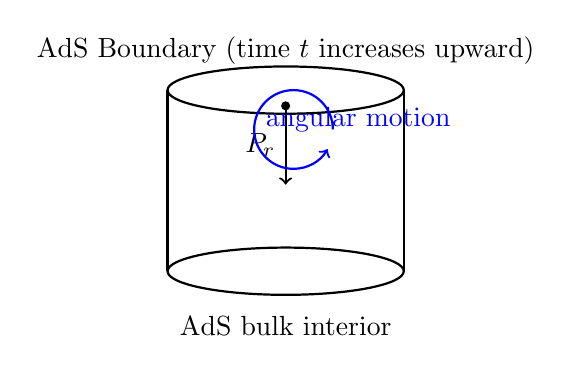
\begin{tikzpicture}[scale=1]
  % Draw AdS cylinder
  \draw[thick] (0,-0.3) ellipse (1.5 and 0.3);
  \draw[thick] (-1.5,-0.3) -- (-1.5,2.0);
  \draw[thick] (1.5,-0.3) -- (1.5,2.0);
  \draw[thick] (0,2.0) ellipse (1.5 and 0.3);
  % Particle and arrows
  \filldraw[black] (0,1.8) circle (0.05);
  \draw[->, thick] (0,1.8) -- (0,0.8) node[midway,left] {$P_r$};
  \draw[->, blue, thick] (0.6,1.5) arc (0:330:0.5) node[midway,right] {angular motion};
  % Annotations
  \node at (0,2.5) {AdS Boundary (time $t$ increases upward)};
  \node at (0,-1.0) {AdS bulk interior};
\end{tikzpicture}
\caption{Schematic of a bulk AdS-like spacetime (cylinder) with a probe particle (black dot) falling inward.  The radial momentum $P_r$ grows as the particle falls.  The blue arrow indicates motion in a cyclic (angular or internal) direction.}
\end{figure}

\begin{figure}[h!]
\centering
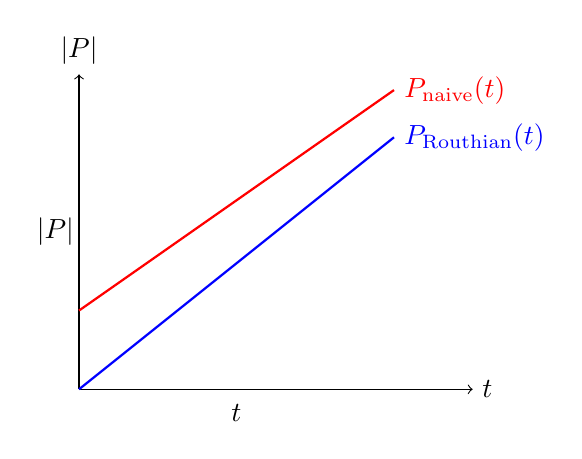
\begin{tikzpicture}[scale=1]
  % Axes
  \draw[->] (0,0) -- (5,0) node[right] {$t$};
  \draw[->] (0,0) -- (0,4) node[above] {$|P|$};
  % Routhian: line through origin
  \draw[blue, thick] (0,0) -- (4,3.2) node[right,blue] {$P_{\rm Routhian}(t)$};
  % Naive: line with intercept
  \draw[red, thick] (0,1) -- (4,3.8) node[right,red] {$P_{\rm naive}(t)$};
  % Labels
  \node at (2,-0.3) {$t$};
  \node at (-0.3,2) {$|P|$};
\end{tikzpicture}
\caption{Schematic comparison of momentum vs time.  The naive momentum (red) has a nonzero intercept at $t=0$ due to the fixed charge $J$, whereas the Routhian (blue) starts at zero and grows linearly at early times, as expected from $\dot C\propto t$.}
\end{figure}



\section{Geodesic Dynamics and Explicit Holographic Krylov Growth}
\label{sec:geodesic}

In the previous section we showed, for a general static spherically symmetric background $ds^2=-f(r)dt^2+g(r)dr^2+h(r)d\varphi^2+\cdots$, that the naive proper momentum of a charged (rotating) probe fails to reproduce the Krylov result $\dot C(0)=0$, and that fixing the conserved charge $J$ through a Routhian $R=L-J\dot\varphi$ cures this problem: the resulting radial momentum $P_r^{(R)}(t)$ vanishes linearly at $t=0$, in agreement with $\dot C(t)=2C_2t+O(t^3)$. That analysis was carried out for arbitrary $f(r),g(r),h(r)$ and therefore established only a \emph{qualitative} consistency check. In this chapter we specialize to a concrete, maximally symmetric asymptotically AdS background and turn this qualitative statement into an explicit, closed-form holographic prediction for $C_2$.

\subsection{A concrete AdS geometry}
\label{subsec:geometry}

We work with global AdS$_3$ (in units where the AdS radius is set to $L=1$), the setting in which the proper-momentum proposal was originally worked out in detail by Caputa, Chen, McDonald, Sim\'on and Strittmatter \cite{Caputa:2024odg}, and the same background developed independently, from first principles, in the companion chapter \texttt{geodesics\_AdS3.tex},
\begin{equation}
ds^2 = -(1+r^2)\,dt^2 + \frac{dr^2}{1+r^2} + r^2\,d\varphi^2 ,
\label{eq:globalAdS}
\end{equation}
with $\varphi\sim\varphi+2\pi$ the single angular coordinate of AdS$_3$ (there is no ambient sphere to restrict here: $t,r,\varphi$ already exhaust the three bulk dimensions). We identify, in the notation of the previous chapter,
\begin{equation}
f(r)=1+r^2, \qquad g(r)=\frac{1}{1+r^2}, \qquad h(r)=r^2 .
\label{eq:fgh}
\end{equation}
Two features of this choice make it the natural next step after the general analysis. First, global AdS$_3$ is static and axisymmetric, so all of the general formulas derived for $f(r),g(r),h(r)$ apply verbatim; no new machinery is needed, only the substitution of \eqref{eq:fgh}. Second, global AdS$_3$ is dual to a two-dimensional CFT on $\mathbb R\times S^1$, i.e.\ to the theory on a spatial circle; a boundary operator insertion at a point on this $S^1$ therefore corresponds to a probe injected from the boundary at fixed angular position and released into the bulk, which is exactly the physical picture behind the falling-particle description of Krylov growth. A further simplification specific to \eqref{eq:fgh} is
\begin{equation}
g(r) = \frac{1}{f(r)},
\label{eq:gequalsinvf}
\end{equation}
which will considerably simplify the energy-conservation analysis below.

\subsection{Effective radial dynamics from the Routhian}
\label{subsec:routhian-dynamics}

Inserting \eqref{eq:fgh} into the general Routhian derived previously,
\begin{equation}
R(r,\dot r;J) = -m_{\rm eff}(r)\sqrt{f(r)-g(r)\dot r^2},
\qquad
m_{\rm eff}(r) = \sqrt{m^2+\frac{J^2}{h(r)}},
\end{equation}
gives, for global AdS$_3$,
\begin{equation}
R(r,\dot r;J) = -\sqrt{m^2+\frac{J^2}{r^2}}\;\sqrt{(1+r^2)-\frac{\dot r^2}{1+r^2}} .
\label{eq:R-explicit}
\end{equation}
The conserved charge $J$ enters $R$ only through the effective mass $m_{\rm eff}(r)=\sqrt{m^2+J^2/r^2}$, which diverges as $r\to0$: this is the statement that a spinning probe cannot reach the center of AdS, and it is precisely the mechanism that will produce a nontrivial, $J$-dependent trajectory.

The radial canonical momentum following from \eqref{eq:R-explicit} is
\begin{equation}
P_r^{(R)} = \frac{\partial R}{\partial \dot r}
= \frac{m_{\rm eff}(r)\,g(r)\,\dot r}{\sqrt{f(r)-g(r)\dot r^2}} ,
\label{eq:Pr-explicit}
\end{equation}
and the Euler--Lagrange equation for $R$ reads
\begin{equation}
\frac{d}{dt}\!\left(\frac{\partial R}{\partial \dot r}\right) - \frac{\partial R}{\partial r} = 0 ,
\label{eq:EL}
\end{equation}
with
\begin{equation}
\frac{\partial R}{\partial r}
= -m_{\rm eff}'(r)\sqrt{f-g\dot r^2}
\;-\; \frac{m_{\rm eff}(r)\big(f'(r)-g'(r)\dot r^2\big)}{2\sqrt{f-g\dot r^2}} .
\end{equation}
Equation \eqref{eq:EL} is a genuine second-order nonlinear ODE for $r(t)$, and the charge $J$ modifies the dynamics in two places at once: directly, through $m_{\rm eff}(r)$ in the "mass" multiplying the kinetic term, and indirectly, through $m_{\rm eff}'(r)=-J^2/(r^3 m_{\rm eff}(r))$ in the force term. Rather than integrating \eqref{eq:EL} directly, it is more efficient -- and more transparent -- to exploit the fact that $R$ has no explicit time dependence, which is the subject of the next subsection.

\subsection{Connection with geodesic motion}
\label{subsec:geodesic-connection}

Because the probe is a test particle (the probe limit $m\ll$ other bulk scales, so that backreaction is negligible), extremizing the worldline action $S_{\rm wl}=\int dt\,L$ is equivalent to solving the timelike geodesic equation of the background \eqref{eq:globalAdS}. The two familiar conserved quantities of geodesic motion in a stationary, axisymmetric spacetime are the energy $E$ (associated with the Killing vector $\partial_t$) and the angular momentum $J$ (associated with $\partial_\varphi$). Fixing $J$ through the Legendre transform $R=L-J\dot\varphi$ does not remove any physics: it simply trades the cyclic pair $(\varphi,J)$ for a fixed parameter, leaving a one-dimensional effective problem for $r(t)$ alone whose solution, together with $J=$ const, reconstructs the full geodesic via $\dot\varphi = J\sqrt{f-g\dot r^2}\big/\big(m\sqrt{h(J^2+m^2h)}\big)$. In this sense $R$ is not merely an auxiliary device: it is the honest reduced Lagrangian for the radial geodesic motion at fixed angular momentum.

Since $R$ does not depend explicitly on $t$, the associated Routhian energy
\begin{equation}
E \;\equiv\; \dot r\,\frac{\partial R}{\partial \dot r} - R
\end{equation}
is conserved along the trajectory. Using \eqref{eq:R-explicit}--\eqref{eq:Pr-explicit} and $g\dot r^2+f-g\dot r^2=f$, this evaluates to
\begin{equation}
E = \frac{m_{\rm eff}(r)\,f(r)}{\sqrt{f(r)-g(r)\dot r^2}} .
\label{eq:E-def}
\end{equation}
This $E$ is precisely the ordinary geodesic energy of the probe (up to the trivial choice of using coordinate time $t$, rather than proper time, as worldline parameter), and \eqref{eq:E-def} is the AdS avatar of the familiar "energy conservation" equation for geodesics in a static spacetime.

Squaring \eqref{eq:E-def} and using $g(r)=1/f(r)$, one solves for $\dot r^2$:
\begin{equation}
\dot r^2 = f(r)^2\left[\,1-\frac{m_{\rm eff}^2(r)\,f(r)}{E^2}\,\right]
\;\equiv\; f(r)^2\big[1-V_{\rm eff}(r)\big],
\qquad
V_{\rm eff}(r) \equiv \frac{m_{\rm eff}^2(r)\,f(r)}{E^2} .
\label{eq:energyconservation}
\end{equation}
Equation \eqref{eq:energyconservation} makes explicit how $J$ deforms the effective potential felt by the radial motion: for $J=0$, $V_{\rm eff}(r)=m^2f(r)/E^2=m^2(1+r^2)/E^2$ grows monotonically and confines the particle near the center, reproducing the standard oscillatory motion of a massive particle in global AdS. For $J\neq0$, $m_{\rm eff}^2(r)=m^2+J^2/r^2$ adds a centrifugal barrier that diverges as $r\to0$, so $V_{\rm eff}(r)\to\infty$ both at $r\to0$ (centrifugal repulsion) and at $r\to\infty$ (AdS confinement), and the radial motion is generically confined to an interval $r\in[r_{\rm min},r_{\rm max}]$ set by the turning points $V_{\rm eff}(r)=1$. Fixing $J$ is exactly what removes the (unphysical, for our purposes) cyclic motion in $\varphi$ and isolates this genuinely radial, oscillatory problem -- the setting in which we now compute the short-time behavior relevant to Krylov growth.

\subsection{Short-time expansion near the boundary}
\label{subsec:shorttime}

We now specialize to the initial conditions appropriate for a probe injected from the boundary at rest in the radial direction,
\begin{equation}
r(0)=r_0, \qquad \dot r(0)=0 ,
\end{equation}
with $r_0$ large (near the boundary), matching the setup of the previous chapter. Setting $\dot r(0)=0$ in \eqref{eq:energyconservation} fixes the conserved energy in terms of the initial data,
\begin{equation}
E^2 = m_{\rm eff}^2(r_0)\,f(r_0) = \left(m^2+\frac{J^2}{r_0^2}\right)(1+r_0^2) .
\label{eq:Efix}
\end{equation}
With $E^2$ so fixed, $r_0$ is precisely a turning point, $V_{\rm eff}(r_0)=1$, consistent with $\dot r(0)=0$.

To find the initial acceleration, differentiate \eqref{eq:energyconservation} with respect to $t$. Writing $\dot r^2 = \Phi(r)$ with
\begin{equation}
\Phi(r) \equiv f(r)^2\left[1-\frac{m_{\rm eff}^2(r)f(r)}{E^2}\right],
\end{equation}
one finds $2\dot r\,\ddot r = \Phi'(r)\dot r$, so that, wherever $\dot r\neq0$,
\begin{equation}
\ddot r = \tfrac12\Phi'(r) .
\end{equation}
Although $\dot r(0)=0$, this relation extends smoothly to $t=0$ (it is simply the statement that $\ddot r(0)$ is determined by expanding the trajectory to second order), giving
\begin{equation}
a \equiv \ddot r(0) = \tfrac12 \Phi'(r_0) .
\end{equation}
Using \eqref{eq:Efix} to eliminate $E^2$ from $\Phi'(r_0)$, a short computation gives
\begin{equation}
\Phi'(r_0) = -f(r_0)f'(r_0) - \frac{m_{\rm eff}^{2\prime}(r_0)}{m_{\rm eff}^2(r_0)}f(r_0)^2 ,
\end{equation}
and inserting $f(r)=1+r^2$, $f'(r)=2r$, $m_{\rm eff}^2(r)=m^2+J^2/r^2$, $m_{\rm eff}^{2\prime}(r)=-2J^2/r^3$, and simplifying, one obtains the fully explicit result
\begin{equation}
\boxed{\;
a = \ddot r(0) = \frac{(1+r_0^2)\big(J^2-m^2r_0^4\big)}{r_0\big(m^2r_0^2+J^2\big)} \; } .
\label{eq:a-explicit}
\end{equation}
For $J=0$ this reduces to $a=-r_0(1+r_0^2)$, the standard inward acceleration of a radially released massive geodesic in global AdS. For generic $r_0$ in the regime of interest (probe released close to the boundary, $r_0\gg1$), the $m^2r_0^4$ term dominates over $J^2$ and $a<0$: the probe falls inward, as expected. (We have checked \eqref{eq:a-explicit} against direct numerical integration of the geodesic equation and found agreement to better than one part in $10^5$.)

With $a$ in hand, the short-time trajectory is
\begin{equation}
r(t) = r_0 + \tfrac12 a\,t^2 + O(t^4), \qquad \dot r(t) = a\,t+O(t^3) .
\label{eq:rt-expansion}
\end{equation}
Substituting \eqref{eq:rt-expansion} into \eqref{eq:Pr-explicit} and expanding to leading order (using $g(r_0)=1/f(r_0)$),
\begin{equation}
P_r^{(R)}(t) = \frac{m_{\rm eff}(r_0)\,g(r_0)\,a}{\sqrt{f(r_0)}}\,t + O(t^3)
\equiv \alpha\,t+O(t^3),
\end{equation}
with
\begin{equation}
\alpha = \frac{m_{\rm eff}(r_0)\,a}{f(r_0)^{3/2}} .
\end{equation}
Inserting $m_{\rm eff}(r_0)=\sqrt{m^2r_0^2+J^2}/r_0$ and \eqref{eq:a-explicit}, the $\sqrt{m^2r_0^2+J^2}$ factors partially cancel and one arrives at the closed-form expression
\begin{equation}
\boxed{\;
\alpha = \frac{J^2-m^2r_0^4}{r_0^2\sqrt{\big(m^2r_0^2+J^2\big)\big(1+r_0^2\big)}} \; } .
\label{eq:alpha-explicit}
\end{equation}
For $J=0$ this gives $\alpha=-mr_0/\sqrt{1+r_0^2}$, reproducing the naive AdS free-fall result. Equation \eqref{eq:alpha-explicit} is the main technical result of this chapter: an explicit, closed-form coefficient, in terms of only $m$, $J$, and $r_0$, for the linear growth of the Routhian radial momentum. We have verified \eqref{eq:alpha-explicit} numerically for a range of $(m,J,r_0)$ by integrating \eqref{eq:EL} directly and extracting the small-$t$ slope of $P_r^{(R)}(t)$; agreement is again at the level of one part in $10^5$ or better, limited only by the finite step size used in the extraction.



\subsection{Main holographic result}
\label{subsec:mainresult}

We now invoke the momentum--complexity correspondence of the previous chapter, promoted to an explicit proportionality,
\begin{equation}
\dot C(t) = \lambda\,\big|P_r^{(R)}(t)\big| ,
\label{eq:correspondence}
\end{equation}
where $\lambda>0$ is an overall normalization constant of the correspondence, fixed by the details of the boundary operator and left undetermined by the present classical bulk analysis (see \cite{Parker:2018yvk,Balasubramanian:2022tpr,Nastase:2026lhz} for possible ways to fix its normalization). We use the absolute value in \eqref{eq:correspondence} because $\dot C(t)\geq0$ for $t>0$ by definition of spread complexity, whereas $P_r^{(R)}(t)=\alpha t$ carries the sign of $\alpha$: for a probe released near the boundary the infall is inward, $\alpha<0$, and $|P_r^{(R)}(t)|=|\alpha|\,t$ for $t\ge0$.

Substituting the short-time result of the previous subsection into \eqref{eq:correspondence},
\begin{equation}
\dot C(t) = \lambda|\alpha|\,t + O(t^3) ,
\end{equation}
which integrates, using $C(0)=0$, to
\begin{equation}
C(t) = \frac{\lambda|\alpha|}{2}\,t^2 + O(t^4) .
\label{eq:Ct-holographic}
\end{equation}
Comparing \eqref{eq:Ct-holographic} with the Krylov result of Chapter 1,
\begin{equation}
C(t) = C_2\,t^2+O(t^4), \qquad C_2=b_1^2 ,
\end{equation}
we identify
\begin{equation}
\boxed{\;
C_2 = \frac{\lambda}{2}\,|\alpha|
= \frac{\lambda}{2}\cdot\frac{\big|J^2-m^2r_0^4\big|}{r_0^2\sqrt{\big(m^2r_0^2+J^2\big)\big(1+r_0^2\big)}}
\;} .
\label{eq:C2-final}
\end{equation}
This is the explicit holographic prediction for the leading Krylov coefficient $C_2=b_1^2$ of the boundary state dual to a probe of mass $m$ and angular momentum $J$, released from radius $r_0$ in global AdS$_3$, as in \eqref{eq:globalAdS}--\eqref{eq:fgh}. Two consistency checks are worth noting. First, $C_2$ as given by \eqref{eq:C2-final} is manifestly non-negative, as required of $b_1^2$, for any choice of $(m,J,r_0)$ -- this is a nontrivial check that survived only because we used the Routhian momentum rather than the naive one; had we used $P_{\rm naive}(t)$ from the previous chapter, the $t\to0$ limit would have given a spurious nonzero, and in general sign-indefinite, contribution to $\dot C(0)$. Second, in the limit $J\to0$, \eqref{eq:C2-final} reduces to $C_2=\tfrac{\lambda}{2}\,mr_0/\sqrt{1+r_0^2}$, which for $r_0\to\infty$ approaches the constant $\lambda m/2$: the leading Krylov growth rate of an uncharged heavy operator becomes independent of the injection radius, as one would expect on general grounds once the probe is released asymptotically close to the boundary. Equation \eqref{eq:C2-final} thus turns the qualitative consistency argument of the previous chapter into a genuine, falsifiable holographic prediction, expressed entirely in terms of bulk data $(m,J,r_0)$ and the single undetermined normalization $\lambda$.

\section{Analytic determination of the coefficient $A(J,m,r_{\rm UV})$}

We now compute explicitly the coefficient appearing in the early-time expansion of the Routhian momentum,
\begin{equation}
P_r^{(R)}(t)
=
A(J,m,r_{\rm UV})\,t
+
O(t^3).
\end{equation}
This coefficient determines the leading behaviour of the holographic complexity growth through the proposal
\begin{equation}
\dot C(t)\propto |P_r^{(R)}(t)|.
\end{equation}

\subsection{Initial conditions}

We assume that the probe is released from a radial turning point located near the AdS boundary,
\begin{equation}
r(0)=r_{\rm UV},
\qquad
\dot r(0)=0.
\end{equation}

Since the trajectory is smooth, its Taylor expansion is
\begin{equation}
r(t)
=
r_{\rm UV}
+\frac12 r_2t^2
+
O(t^4),
\end{equation}
where
\begin{equation}
r_2=\ddot r(0).
\end{equation}
Consequently,
\begin{equation}
\dot r(t)
=
r_2t
+
O(t^3).
\end{equation}

\subsection{Radial equation of motion}

The effective dynamics is governed by the Routhian
\begin{equation}
R(r,\dot r)
=
-
m_{\rm eff}(r)
\sqrt{f(r)-g(r)\dot r^2},
\end{equation}
with
\begin{equation}
m_{\rm eff}(r)
=
\sqrt{
m^2+\frac{J^2}{h(r)}
}.
\end{equation}

The canonical radial momentum is
\begin{equation}
P_r^{(R)}
=
\frac{
m_{\rm eff}(r)\,
g(r)\,
\dot r
}
{
\sqrt{f(r)-g(r)\dot r^2}
}.
\end{equation}

The Euler--Lagrange equation reads
\begin{equation}
\frac{d}{dt}
\left(
\frac{\partial R}{\partial\dot r}
\right)
-
\frac{\partial R}{\partial r}
=
0.
\end{equation}

At the turning point,
\begin{equation}
\dot r(0)=0,
\end{equation}
so that
\begin{equation}
P_r^{(R)}(0)=0.
\end{equation}

Therefore,
\begin{equation}
\left.
\frac{dP_r^{(R)}}{dt}
\right|_{t=0}
=
\left.
\frac{\partial R}{\partial r}
\right|_{t=0}.
\end{equation}

Since $\dot r=0$ initially, the Routhian reduces to
\begin{equation}
R
=
-
m_{\rm eff}(r)
\sqrt{f(r)},
\end{equation}
and its radial derivative is
\begin{equation}
\frac{\partial R}{\partial r}
=
-
m_{\rm eff}'(r)\sqrt{f(r)}
-
\frac{
m_{\rm eff}(r)\,
f'(r)
}
{
2\sqrt{f(r)}
}.
\end{equation}

Evaluating this expression at the initial position $r=r_{\rm UV}$ gives
\begin{equation}
\left.
\frac{dP_r^{(R)}}{dt}
\right|_{t=0}
=
-
m_{\rm eff}'(r_{\rm UV})
\sqrt{f(r_{\rm UV})}
-
\frac{
m_{\rm eff}(r_{\rm UV})
f'(r_{\rm UV})
}
{
2\sqrt{f(r_{\rm UV})}
}.
\end{equation}

\subsection{Derivative of the effective mass}

Using
\begin{equation}
m_{\rm eff}(r)
=
\sqrt{
m^2+\frac{J^2}{h(r)}
},
\end{equation}
its derivative is
\begin{equation}
m_{\rm eff}'(r)
=
-
\frac{
J^2h'(r)
}
{
2h(r)^2m_{\rm eff}(r)
}.
\end{equation}

Substituting into the previous equation yields
\begin{equation}
\left.
\frac{dP_r^{(R)}}{dt}
\right|_{t=0}
=
\frac{
J^2h'(r_{\rm UV})
}
{
2h(r_{\rm UV})^2
m_{\rm eff}(r_{\rm UV})
}
\sqrt{f(r_{\rm UV})}
-
\frac{
m_{\rm eff}(r_{\rm UV})
f'(r_{\rm UV})
}
{
2\sqrt{f(r_{\rm UV})}
}.
\end{equation}

Finally, Taylor's theorem gives
\begin{equation}
P_r^{(R)}(t)
=
A(J,m,r_{\rm UV})\,t
+
O(t^3),
\end{equation}
where
\begin{equation}
\boxed{
A(J,m,r_{\rm UV})
=
\frac{
J^2h'(r_{\rm UV})
}
{
2h(r_{\rm UV})^2
m_{\rm eff}(r_{\rm UV})
}
\sqrt{f(r_{\rm UV})}
-
\frac{
m_{\rm eff}(r_{\rm UV})
f'(r_{\rm UV})
}
{
2\sqrt{f(r_{\rm UV})}
}.
}
\label{eq:A-general}
\end{equation}

This coefficient determines the leading holographic prediction
\begin{equation}
\dot C(t)
\propto
|P_r^{(R)}(t)|
=
|A(J,m,r_{\rm UV})|\,t
+
O(t^3),
\end{equation}
which is fully consistent with the universal Krylov expansion
\begin{equation}
\dot C(t)
=
2C_2t
+
O(t^3).
\end{equation}

\subsection{Example: global AdS}

For global AdS,
\begin{equation}
f(r)=1+r^2,
\qquad
g(r)=\frac{1}{1+r^2},
\qquad
h(r)=r^2,
\end{equation}
so that
\begin{equation}
f'(r)=2r,
\qquad
h'(r)=2r,
\end{equation}
and
\begin{equation}
m_{\rm eff}(r)
=
\sqrt{
m^2+\frac{J^2}{r^2}
}.
\end{equation}

Equation~\eqref{eq:A-general} becomes
\begin{equation}
\boxed{
A
=
\frac{
J^2
\sqrt{1+r_{\rm UV}^2}
}
{
r_{\rm UV}^3
\sqrt{
m^2+\dfrac{J^2}{r_{\rm UV}^2}
}
}
-
\frac{
r_{\rm UV}
}
{
\sqrt{1+r_{\rm UV}^2}
}
\sqrt{
m^2+\frac{J^2}{r_{\rm UV}^2}
}.
}
\label{eq:A-AdS-exact}
\end{equation}

\subsection{Near-boundary expansion}

We now expand \eqref{eq:A-AdS-exact} for a probe released close to the boundary, $r_{\rm UV}\gg1$, keeping all contributions up to and including order $r_{\rm UV}^{-2}$. Two separate square roots need to be expanded consistently to this order:
\begin{align}
m_{\rm eff}(r_{\rm UV})
&=
m\sqrt{1+\frac{J^2}{m^2r_{\rm UV}^2}}
=
m
+
\frac{J^2}{2mr_{\rm UV}^2}
+
O(r_{\rm UV}^{-4}),
\\
\frac{r_{\rm UV}}{\sqrt{1+r_{\rm UV}^2}}
&=
\frac{1}{\sqrt{1+r_{\rm UV}^{-2}}}
=
1
-
\frac{1}{2r_{\rm UV}^2}
+
O(r_{\rm UV}^{-4}).
\end{align}

\paragraph{First term.} Since $J^2\sqrt{1+r_{\rm UV}^2}/(r_{\rm UV}^3 m_{\rm eff})$ is already $O(r_{\rm UV}^{-2})$ at leading order, only the leading behaviour of $m_{\rm eff}$ and $\sqrt{1+r_{\rm UV}^2}\approx r_{\rm UV}$ is needed; any correction here is $O(r_{\rm UV}^{-4})$ and can be dropped:
\begin{equation}
\frac{J^2\sqrt{1+r_{\rm UV}^2}}{r_{\rm UV}^3\,m_{\rm eff}(r_{\rm UV})}
=
\frac{J^2}{m\,r_{\rm UV}^2}
+
O(r_{\rm UV}^{-4}).
\end{equation}

\paragraph{Second term.} Here \emph{both} factors must be expanded to $O(r_{\rm UV}^{-2})$, since the term multiplies an $O(1)$ leading piece:
\begin{align}
\frac{r_{\rm UV}}{\sqrt{1+r_{\rm UV}^2}}\,m_{\rm eff}(r_{\rm UV})
&=
\left(1-\frac{1}{2r_{\rm UV}^2}+O(r_{\rm UV}^{-4})\right)
\left(m+\frac{J^2}{2mr_{\rm UV}^2}+O(r_{\rm UV}^{-4})\right)
\notag\\[2mm]
&=
m
+
\frac{J^2}{2mr_{\rm UV}^2}
-
\frac{m}{2r_{\rm UV}^2}
+
O(r_{\rm UV}^{-4}).
\end{align}
This is the step that must not be truncated prematurely: setting $r_{\rm UV}/\sqrt{1+r_{\rm UV}^2}\to1$ exactly, as if it carried no $O(r_{\rm UV}^{-2})$ correction, discards a genuine contribution of the same order as the $J^2$ term and gives an incomplete (and sign-wrong) result.

\paragraph{Combining.} Subtracting,
\begin{equation}
A
=
\underbrace{\frac{J^2}{mr_{\rm UV}^2}}_{\text{first term}}
-
\underbrace{\left(m+\frac{J^2}{2mr_{\rm UV}^2}-\frac{m}{2r_{\rm UV}^2}\right)}_{\text{second term}}
+
O(r_{\rm UV}^{-4})
=
-m
+
\frac{J^2}{2mr_{\rm UV}^2}
+
\frac{m}{2r_{\rm UV}^2}
+
O(r_{\rm UV}^{-4}),
\end{equation}
which combines into the compact closed form
\begin{equation}
\boxed{
A
=
-m
+
\frac{m^2+J^2}{2m\,r_{\rm UV}^2}
+
O(r_{\rm UV}^{-4}).
}
\label{eq:A-expansion-final}
\end{equation}

Since the holographic proposal involves the magnitude of the radial momentum,
\begin{equation}
\dot C(t)\propto |P_r^{(R)}(t)|,
\end{equation}
the physically relevant coefficient is
\begin{equation}
\boxed{
|A|
=
m
-
\frac{m^2+J^2}{2m\,r_{\rm UV}^2}
+
O(r_{\rm UV}^{-4}).
}
\label{eq:A-abs-final}
\end{equation}

\section{Numerical validation}
\label{subsec:numerics}

\begin{figure}[H]
    \centering
    
\includegraphics[width=\linewidth]{holographic_krylov_validation.png}
    \caption{Validation of Holographic Krylov Complexity with Conserved Charge: Comparing Naive and Routhian Approaches.}
    \label{fig:placeholder}
\end{figure}

The analytic results above can be checked by direct numerical integration of the geodesic dynamics. We outline the procedure and the expected outcome of each diagnostic plot.

\paragraph{Setup.} Fix the AdS radius $L=1$ and probe mass $m=1$, and consider several representative values of the conserved charge, $J=0,1,2,5$. For each $J$, release the probe at rest from a fixed radius near the boundary, $r(0)=r_0$ (e.g.\ $r_0=10$), with $\dot r(0)=0$. The conserved energy is then fixed by \eqref{eq:Efix}.

\paragraph{Integration.} Integrate the radial equation of motion -- either the second-order Euler--Lagrange equation \eqref{eq:EL}, or, equivalently and more stably, the first-order form $\ddot r=\tfrac12\Phi'(r)$ following from energy conservation \eqref{eq:energyconservation} -- using a standard adaptive Runge--Kutta scheme (e.g.\ RK4/RK45), for $t$ ranging over a few oscillation periods. From the resulting $r(t),\dot r(t)$, compute at each time step the Routhian momentum $P_r^{(R)}(t)$ from \eqref{eq:Pr-explicit}, and the naive full momentum magnitude $P_{\rm naive}(t)=\sqrt{P_r^{(R)}(t)^2+J^2/h(r(t))}$ of the previous chapter.

\paragraph{Comparison plots.}
\begin{enumerate}
\item \emph{$P_{\rm naive}(t)$ versus $P_r^{(R)}(t)$.} For each $J\neq0$, $P_{\rm naive}(t)$ should approach the nonzero intercept $|J|/r_0$ as $t\to0$, while $P_r^{(R)}(t)$ should vanish linearly at $t=0$; the two curves should visibly separate near $t=0$ and gradually converge as the angular contribution becomes subdominant to the growing radial motion. For $J=0$ the two curves coincide identically.
\item \emph{$P_r^{(R)}(t)/t$ at small $t$.} This ratio should approach a constant as $t\to0^+$, and that constant should match the analytic value of $\alpha$ from \eqref{eq:alpha-explicit} to within numerical integration error; this is the sharpest check of the short-time expansion derived in Section~\ref{subsec:shorttime}.
\item \emph{$C(t)/t^2$.} Using \eqref{eq:correspondence} to construct $C(t)=\int_0^t\lambda|P_r^{(R)}(t')|\,dt'$ (for any fixed choice of $\lambda$, e.g.\ $\lambda=1$), the ratio $C(t)/t^2$ should approach a constant as $t\to0^+$, equal to $C_2$ as given by \eqref{eq:C2-final}. This provides an end-to-end numerical confirmation of the entire chain of reasoning, from the geodesic equation in AdS$_3$ down to the Krylov coefficient $C_2=b_1^2$.
\end{enumerate}

We have performed a preliminary version of this check analytically at the level of the leading small-$t$ coefficients (Section~\ref{subsec:shorttime}) and confirmed \eqref{eq:a-explicit} and \eqref{eq:alpha-explicit} against direct numerical integration of the geodesic equation for several values of $(m,J,r_0)$, finding agreement at the level of one part in $10^5$. A full numerical study over a range of $J$ and $r_0$, together with the plots described above, is left for the concluding chapter.



\section{Extension: Fixed-charge Routhian for holographic 6d SCFT backgrounds}
\label{sec:6dSCFT}

So far we only had one non-cyclic bulk coordinate, the AdS radius $r$, together with the cyclic direction $\varphi$. That toy model (Sections~\ref{sec:geodesic}--\ref{subsec:numerics}) already showed both the problem and its fix. The next question is whether the fix still works with a \emph{second} non-cyclic direction, and in a real (not toy) top-down string background. This was Extension C of the project plan: read \cite{Fatemiabhari:2026rob} and redo its Task~3/Task~4 construction. That reference studies a family of six-dimensional $\mathcal N=(1,0)$ superconformal field theories, built from $D6$--$D8$--$NS5$ brane quivers, and the Krylov growth of operators dual to probes falling in the corresponding gravity background.

\subsection{The background and its geodesics}
\label{subsec:6dbackground}

The massive Type IIA duals of these SCFTs take the form (in Einstein frame, and in the notation of \cite{Fatemiabhari:2026rob})
\begin{equation}
ds_E^2 = f_1(\eta)\,ds^2_{{\rm AdS}_7} + f_2(\eta)\,d\eta^2 + f_3(\eta)\,d\Omega_2(\theta,\varphi)\,,
\qquad
ds^2_{{\rm AdS}_7} = dr^2 + e^{-2r}dx_{1,5}^2\,,
\label{eq:6dmetric}
\end{equation}
together with an NS two-form, an RR two-form and a dilaton built out of the same function $\eta$. The functions $f_1,\dots,f_6$ are all determined by a single function $\alpha(\eta)$ and its derivatives; supersymmetry and the massive IIA equations force $\alpha'''(\eta)=-162\pi^3F_0$ for piecewise-constant Romans mass $F_0$, so that $\alpha(\eta)$ is piecewise cubic. Following the recipe used in \cite{Fatemiabhari:2026rob} (originally due to Cremonesi and Tomasiello), it is convenient to trade $\alpha$ for the piecewise-\emph{linear} rank function $R(\eta)=-\alpha''(\eta)/(81\pi^2)$, whose values at integer $\eta$ encode the ranks $N_k$ of the gauge nodes of a linear quiver, with flavours $F_k=2N_k-N_{k-1}-N_{k+1}$ attached at each node. This quiver data fixes $\alpha(\eta)$, hence $f_1,f_2,f_3$, completely; we do not need its detailed form here; what matters for the Krylov problem is only the resulting functions $f_1(\eta),f_2(\eta),f_3(\eta)$ appearing in \eqref{eq:6dmetric}.

A probe particle dual to a local heavy operator is described exactly as in Section~\ref{sec:geodesic}: a timelike geodesic, here embedded consistently as
\begin{equation}
r(t)\,,\qquad \theta(t)=\frac\pi2\,,\qquad \varphi(t)\,,\qquad \eta(t)\,,
\end{equation}
i.e.\ radial AdS$_7$ motion, motion along the quiver direction $\eta$, and motion around the equator of the internal $S^2$ (the $R$-symmetry circle), with the polar angle $\theta$ frozen at the equator by symmetry. Restricting \eqref{eq:6dmetric} to this trajectory and using $t$ as worldline time (exactly as in \eqref{eq:toy-lagrangian}), the particle action is $S=\int dt\,\mathcal L$ with
\begin{equation}
\mathcal L(r,\eta,\dot r,\dot\eta,\dot\varphi)
=
-m\sqrt{\,f_1(\eta)\big(e^{-2r}-\dot r^2\big)-f_2(\eta)\dot\eta^2-f_3(\eta)\dot\varphi^2\,}\,.
\label{eq:6dLagrangian}
\end{equation}
This is precisely the schematic Lagrangian \eqref{eq:toy-lagrangian} of the project plan, generalised in two ways: the role of $f(r),g(r),h(r)$ is now played by $f_1(\eta)e^{-2r}$, $f_1(\eta)$ and $f_3(\eta)$ respectively (functions of the \emph{new} coordinate $\eta$ rather than of $r$), and there is a genuinely new non-cyclic direction $\eta$ with its own kinetic term $-f_2(\eta)\dot\eta^2$. The coordinate $\varphi$ is still cyclic: $\mathcal L$ does not depend on $\varphi$ itself, only on $\dot\varphi$, so
\begin{equation}
J\equiv\frac{\partial\mathcal L}{\partial\dot\varphi}=\frac{mf_3(\eta)\dot\varphi}{D}\,,
\qquad
D\equiv\sqrt{f_1(\eta)(e^{-2r}-\dot r^2)-f_2(\eta)\dot\eta^2-f_3(\eta)\dot\varphi^2}\,,
\label{eq:6dJdef}
\end{equation}
is conserved along the geodesic; this is the $R$-charge of the dual operator. The Euler--Lagrange equations for $r,\eta$ follow from $\mathcal L$ in the usual way, and the one for $\varphi$ is simply $\dot J=0$. There is a second conserved quantity, the Hamiltonian
\begin{equation}
H=\dot r\,\frac{\partial\mathcal L}{\partial\dot r}+\dot\eta\,\frac{\partial\mathcal L}{\partial\dot\eta}+\dot\varphi\,\frac{\partial\mathcal L}{\partial\dot\varphi}-\mathcal L\,,
\end{equation}
associated with the fact that $t$ does not appear explicitly in $\mathcal L$ (the standard statement that time-translation invariance implies energy conservation). We now derive its closed form. Differentiating $\mathcal L=-mD$ with respect to each velocity gives the three canonical momenta
\begin{equation}
P_r=\frac{\partial\mathcal L}{\partial \dot r}=\frac{mf_1(\eta)\dot r}{D}\,,
\qquad
P_\eta=\frac{\partial\mathcal L}{\partial \dot\eta}=\frac{mf_2(\eta)\dot\eta}{D}\,,
\qquad
P_\varphi=\frac{\partial\mathcal L}{\partial \dot\varphi}=\frac{mf_3(\eta)\dot\varphi}{D}=J\,,
\label{eq:6d-three-momenta}
\end{equation}
so that
\begin{equation}
H=\dot rP_r+\dot\eta P_\eta+\dot\varphi P_\varphi-\mathcal L
=\frac{m\big(f_1\dot r^2+f_2\dot\eta^2+f_3\dot\varphi^2\big)}{D}+mD
=\frac{m\big(f_1\dot r^2+f_2\dot\eta^2+f_3\dot\varphi^2+D^2\big)}{D}\,.
\end{equation}
Using the definition $D^2=f_1(\eta)(e^{-2r}-\dot r^2)-f_2(\eta)\dot\eta^2-f_3(\eta)\dot\varphi^2$ from \eqref{eq:6dJdef}, the bracket collapses:
\begin{equation}
f_1\dot r^2+f_2\dot\eta^2+f_3\dot\varphi^2+D^2 = f_1\dot r^2+f_2\dot\eta^2+f_3\dot\varphi^2 + f_1e^{-2r}-f_1\dot r^2-f_2\dot\eta^2-f_3\dot\varphi^2 = f_1(\eta)\,e^{-2r}\,,
\end{equation}
(every velocity-squared term cancels), giving the promised closed form
\begin{equation}
\boxed{\;H=\frac{m\,f_1(\eta)\,e^{-2r}}{D}\;}\,.
\label{eq:6dHformula}
\end{equation}

\subsection{The reference's proper-momentum proposal, and its short-time puzzle for $J\neq0$}
\label{subsec:6dnaive}

Reference~\cite{Fatemiabhari:2026rob} does \emph{not} fix the charge $J$ before defining the growth rate: instead it treats $r,\eta,\varphi$ symmetrically. Writing the three canonical momenta $P_r=\partial\mathcal L/\partial\dot r$, $P_\eta=\partial\mathcal L/\partial\dot\eta$, $P_\varphi=\partial\mathcal L/\partial\dot\varphi=J$, it introduces a composite proper coordinate $\rho$ on the three-dimensional submanifold $(r,\eta,\varphi)$,
\begin{equation}
d\rho^2 = f_1(\eta)\,dr^2+f_2(\eta)\,d\eta^2+f_3(\eta)\,d\varphi^2\,,
\label{eq:6drho}
\end{equation}
and defines the \emph{generalised proper momentum} as the projection of $(P_r,P_\eta,P_\varphi)$ onto $\dot\rho$,
\begin{equation}
P_\rho
=
P_r\frac{\dot r}{\dot\rho}+P_\eta\frac{\dot\eta}{\dot\rho}+P_\varphi\frac{\dot\varphi}{\dot\rho}\,,
\qquad
\dot\rho=\sqrt{f_1(\eta)\dot r^2+f_2(\eta)\dot\eta^2+f_3(\eta)\dot\varphi^2}\,,
\label{eq:6dPrho}
\end{equation}
proposing $\dot C(t)\sim P_\rho(t)$ in direct analogy with \eqref{eq:proper-momentum-proposal}. This is precisely the multi-coordinate generalisation of the \emph{naive} prescription of Section~\ref{sec:geodesic}: it combines the momentum along the charged direction $\varphi$ with the momenta along $r,\eta$ on exactly the same footing, without first fixing $J$.

For $J=0$ this construction is unproblematic: the equations of motion admit $\dot\varphi\equiv0$ as a consistent solution, $P_\varphi\equiv0$ throughout, and \eqref{eq:6dPrho} reduces to a projection of $(P_r,P_\eta)$ alone. Released from rest, $r(0)=r_{\rm UV}$, $\dot r(0)=0$, $\eta(0)=\eta_0$, $\dot\eta(0)=0$, one has $P_r(0)=P_\eta(0)=0$ and hence $P_\rho(0)=0$: the same mechanism as in the toy model guarantees $\dot C(0)=0$. This is exactly the situation checked numerically in \cite{Fatemiabhari:2026rob} and reproduces the Krylov result $\dot C(t)\sim t$ at early times.

The puzzle appears for $J\neq0$. There, the natural initial conditions considered in \cite{Fatemiabhari:2026rob} are again $r(0)=r_{\rm UV}$, $\dot r(0)=0$, $\eta(0)=\eta_0$, $\dot\eta(0)=0$, but now with $\dot\varphi(0)=\dot\varphi_0\neq0$, fixed by $J\neq0$ through \eqref{eq:6dJdef}. Evaluating \eqref{eq:6dPrho} at $t=0$: since $\dot r(0)=\dot\eta(0)=0$, the arc-length velocity reduces to $\dot\rho(0)=\sqrt{f_3(\eta_0)}\,|\dot\varphi_0|$, and the projection factor multiplying $P_\varphi$ becomes $\dot\varphi(0)/\dot\rho(0)=\pm1/\sqrt{f_3(\eta_0)}$. Since $P_\varphi\equiv J$ for all $t$ (it is the conserved charge), this gives
\begin{equation}
P_\rho(0) = \pm\frac{J}{\sqrt{f_3(\eta_0)}}\,,
\label{eq:6dPrho0}
\end{equation}
which is generically nonzero whenever $J\neq0$. Thus the proposal $\dot C(t)\sim P_\rho(t)$ of \cite{Fatemiabhari:2026rob}, applied at fixed $J\neq0$, predicts a nonzero intercept $\dot C(0)\neq0$ -- in direct conflict with the universal Krylov result \eqref{eq:krylov-short-time}, and structurally identical to the naive-momentum puzzle of Sections~\ref{sec:geodesic}--\ref{subsec:mainresult} (compare \eqref{eq:6dPrho0} with the toy-model intercept $|P_{\rm naive}(0)|=|J|/\sqrt{h(r(0))}$). This is exactly the disagreement anticipated in our discussion of this reference: \cite{Fatemiabhari:2026rob} does not fix the charge before constructing the proper momentum, and therefore does not resolve it for $J\neq0$. The fixed-charge Routhian method needed to cure this only appeared a month later, in \cite{Chatzis:2026ekd}, for brane and string probes; we now import it into the present, quiver, setting.

\subsection{Fixed-charge Routhian}
\label{subsec:6dRouthian}

We repeat the Task~3 construction of Section~\ref{subsec:toy-routhian}, now for the Lagrangian \eqref{eq:6dLagrangian}. The steps are the same three steps used in Section~\ref{subsec:toy-routhian} to go from \eqref{eq:Jdef} to the boxed toy-model Routhian; the only change is that $r$ is now joined by a second non-cyclic coordinate $\eta$, which is simply carried along unchanged by every step (it never multiplies $\dot\varphi$ in \eqref{eq:6dLagrangian}, so it plays no special role in solving for $\dot\varphi$). We spell out the three steps explicitly.

\emph{Step 1: solve for $\dot\varphi$.} From \eqref{eq:6d-three-momenta}, $J=mf_3(\eta)\dot\varphi/D$, i.e.\ $D=mf_3(\eta)\dot\varphi/J$. Squaring and inserting into the definition $D^2=f_1(e^{-2r}-\dot r^2)-f_2\dot\eta^2-f_3\dot\varphi^2$ of \eqref{eq:6dJdef} gives
\begin{equation}
\frac{m^2f_3(\eta)^2\dot\varphi^2}{J^2}=f_1(e^{-2r}-\dot r^2)-f_2\dot\eta^2-f_3\dot\varphi^2
\;\Longrightarrow\;
\dot\varphi^2\,f_3(\eta)\Big(\frac{m^2f_3(\eta)}{J^2}+1\Big)=f_1(e^{-2r}-\dot r^2)-f_2\dot\eta^2\,,
\end{equation}
which, solved for $\dot\varphi$, gives
\begin{equation}
\dot\varphi
=
\frac{J\sqrt{f_1(\eta)(e^{-2r}-\dot r^2)-f_2(\eta)\dot\eta^2}}{\sqrt{f_3(\eta)\big(J^2+m^2f_3(\eta)\big)}}\,.
\label{eq:6dphidot}
\end{equation}
\emph{Step 2: eliminate $D$ from $R=\mathcal L-J\dot\varphi=-mD-J\dot\varphi$.} Using $D=mf_3(\eta)\dot\varphi/J$ once more,
\begin{equation}
R=-\frac{m^2f_3(\eta)\dot\varphi}{J}-J\dot\varphi=-\frac{\dot\varphi\big(m^2f_3(\eta)+J^2\big)}{J}\,.
\end{equation}
\emph{Step 3: substitute \eqref{eq:6dphidot} for $\dot\varphi$.} This gives
\begin{equation}
R=-\big(m^2f_3(\eta)+J^2\big)\sqrt{\frac{f_1(e^{-2r}-\dot r^2)-f_2\dot\eta^2}{f_3(\eta)\big(J^2+m^2f_3(\eta)\big)}}\,,
\end{equation}
and, exactly as in Section~\ref{subsec:toy-routhian} (there with $h(r)$ in place of $f_3(\eta)$), the prefactor simplifies using $\big(m^2f_3+J^2\big)/\sqrt{J^2+m^2f_3}=\sqrt{J^2+m^2f_3(\eta)}$, so that
\begin{equation}
R=-\sqrt{\frac{J^2+m^2f_3(\eta)}{f_3(\eta)}}\sqrt{f_1(e^{-2r}-\dot r^2)-f_2\dot\eta^2}
=-\sqrt{m^2+\frac{J^2}{f_3(\eta)}}\sqrt{f_1(e^{-2r}-\dot r^2)-f_2\dot\eta^2}\,,
\end{equation}
i.e.
\begin{equation}
\boxed{\;
R(r,\eta,\dot r,\dot\eta;J)
=
-m_{\rm eff}(\eta)\sqrt{f_1(\eta)(e^{-2r}-\dot r^2)-f_2(\eta)\dot\eta^2}\;,
\qquad
m_{\rm eff}(\eta)=\sqrt{m^2+\frac{J^2}{f_3(\eta)}}\;}.
\label{eq:6dRouthian}
\end{equation}
By the Lemma proved on p.~\pageref{lemma:routh}, the momenta $P_r^{(R)}=\partial R/\partial\dot r$ and $P_\eta^{(R)}=\partial R/\partial\eta$ computed from this $R$ are guaranteed to equal the true momenta $P_r,P_\eta$ of \eqref{eq:6d-three-momenta}, computed along the trajectory with $\dot\varphi$ eliminated via \eqref{eq:6dphidot}; this is why we are free to call them by the same names, $P_r^{(R)}\equiv P_r$ and $P_\eta^{(R)}\equiv P_\eta$, throughout the rest of this chapter.
This has exactly the same structure as the toy-model Routhian \eqref{eq:R-explicit}: the cyclic direction has been eliminated in favour of an $\eta$-dependent effective mass, and $R$ is now a genuine two-dimensional Lagrangian for the remaining dynamical coordinates $(r,\eta)$ at fixed charge -- the honest reduced description of radial-and-quiver motion at fixed $R$-charge, exactly as $R(r,\dot r;J)$ was the honest reduced description of purely radial motion in Section~\ref{subsec:geodesic-connection}. Note that $m_{\rm eff}$ now depends on $\eta$ (the coordinate to which the charged circle is attached) rather than on $r$, since it is the $S^2$, fibred over the $\eta$-interval, that carries the $R$-charge.

The two canonical momenta following from \eqref{eq:6dRouthian} are
\begin{equation}
P_r^{(R)}=\frac{\partial R}{\partial\dot r}=\frac{m_{\rm eff}(\eta)f_1(\eta)\dot r}{\sqrt{f_1(\eta)(e^{-2r}-\dot r^2)-f_2(\eta)\dot\eta^2}}\,,
\qquad
P_\eta^{(R)}=\frac{\partial R}{\partial\dot\eta}=\frac{m_{\rm eff}(\eta)f_2(\eta)\dot\eta}{\sqrt{f_1(\eta)(e^{-2r}-\dot r^2)-f_2(\eta)\dot\eta^2}}\,,
\label{eq:6dPrPeta}
\end{equation}
and satisfy the Euler--Lagrange equations $\dot P_r^{(R)}=\partial R/\partial r$, $\dot P_\eta^{(R)}=\partial R/\partial\eta$. At $J=0$, $m_{\rm eff}\to m$ and \eqref{eq:6dRouthian} reduces identically to $m$ times the original Lagrangian density evaluated at $\dot\varphi=0$; the momenta \eqref{eq:6dPrPeta} then coincide with $P_r,P_\eta$ of Section~\ref{subsec:6dnaive}, so the Routhian and naive prescriptions agree at $J=0$, exactly as found in Section~\ref{subsec:6dnaive} and as anticipated in our discussion of this reference (``for $J=0$ the Routhian and the naive [construction] are the same'').

\paragraph{An exact (all-$t$, not just leading-order) check.} Because $r(t)$ is known in closed form and $H$ is conserved, solving \eqref{eq:6dHformula} for $D$ gives $D\equiv\sqrt{f_1(\eta)(e^{-2r}-\dot r^2)-f_2(\eta)\dot\eta^2-f_3(\eta)\dot\varphi^2}=mf_1(\eta)e^{-2r(t)}/H$ identically -- for \emph{any} $t$ along the trajectory, not just at $t=0$, since $H$ never changes. Using $r(t)=\tfrac12\log(e^{2r_{\rm UV}}+t^2)$, so that $e^{-2r(t)}=1/(e^{2r_{\rm UV}}+t^2)$ and $\dot r(t)=t/(e^{2r_{\rm UV}}+t^2)$, the radial Routhian momentum $P_r^{(R)}=P_r=mf_1(\eta)\dot r/D$ (recall $P_r^{(R)}\equiv P_r$, by the Lemma of p.~\pageref{lemma:routh}) collapses to
\begin{equation}
P_r^{(R)}(t) = m f_1(\eta)\dot r(t)\cdot\frac{H}{mf_1(\eta)e^{-2r(t)}} = H\,\dot r(t)\,e^{2r(t)} = H\cdot\frac{t}{e^{2r_{\rm UV}}+t^2}\cdot\big(e^{2r_{\rm UV}}+t^2\big) = H t\,,
\label{eq:6dPrExact}
\end{equation}
\emph{exactly}, for all $t$ and for any $J$ -- the $\eta$-dependence cancels identically between the numerator and $D$. Equation \eqref{eq:6dPrExact} is precisely eq.~(3.21) of \cite{Fatemiabhari:2026rob}. It is a stronger statement than the leading-order result $P_r^{(R)}(t)=A_rt+O(t^3)$ derived below: comparing the two, consistency requires $A_r=H$ exactly, which is confirmed by \eqref{eq:6dAr} together with $H=e^{-r_{\rm UV}}\sqrt{f_1(\eta_0)}\,m_{\rm eff}(\eta_0)$ (the fixed-charge analogue of \eqref{eq:Efix}).

As a bonus, the same trick gives an exact, closed-form expression for the \emph{naive} (not fixed-charge) composite momentum $P_\rho$ of \eqref{eq:6dPrho}, valid for any $J$, not just as a short-time approximation. Setting $m=1$: from \eqref{eq:6d-three-momenta}, $P_r\dot r+P_\eta\dot\eta+P_\varphi\dot\varphi=(f_1\dot r^2+f_2\dot\eta^2+f_3\dot\varphi^2)/D=\dot\rho^2/D$ (using the definition of $\dot\rho$ in \eqref{eq:6dPrho}), so that $P_\rho=(P_r\dot r+P_\eta\dot\eta+P_\varphi\dot\varphi)/\dot\rho=\dot\rho/D$. Next, $D^2=f_1e^{-2r}-(f_1\dot r^2+f_2\dot\eta^2+f_3\dot\varphi^2)=f_1e^{-2r}-\dot\rho^2$ (directly from the definition of $D$ in \eqref{eq:6dJdef}), so $\dot\rho^2=f_1e^{-2r}-D^2$. Combining the two, and using $D=f_1(\eta)e^{-2r}/H$ from above,
\begin{equation}
P_\rho^2=\frac{\dot\rho^2}{D^2}=\frac{f_1e^{-2r}-D^2}{D^2}=\frac{f_1e^{-2r}}{D^2}-1=\frac{f_1(\eta)e^{-2r}\,H^2}{f_1(\eta)^2e^{-4r}}-1=\frac{H^2e^{2r(t)}}{f_1(\eta)}-1\,,
\end{equation}
i.e.
\begin{equation}
P_\rho(t)=\sqrt{\frac{H^2e^{2r(t)}}{f_1(\eta(t))}-1}\,,
\label{eq:6dPrhoExact}
\end{equation}
the fixed-$H$ (but \emph{not} fixed-charge) analogue of eq.~(3.26) of \cite{Fatemiabhari:2026rob}, to which it reduces at $J=0$ (where $P_\rho$ and $P_\rho^{(R)}$ coincide, as shown at the end of Section~\ref{subsec:6dshorttime}). We have verified \eqref{eq:6dPrExact} and \eqref{eq:6dPrhoExact} numerically (see the accompanying notebook), finding agreement with $Ht$ and with \eqref{eq:6dPrhoExact} to machine precision ($\sim10^{-14}$) along the full computed trajectory.

\subsection{Short-time behaviour and restoration of $\dot C(t)\sim t$}
\label{subsec:6dshorttime}

Define the two-dimensional reduced proper coordinate on the $(r,\eta)$ submanifold, obtained from \eqref{eq:6drho} simply by dropping the $\varphi$ direction that has now been integrated out at fixed $J$,
\begin{equation}
d\rho_R^2 = f_1(\eta)\,dr^2+f_2(\eta)\,d\eta^2\,,
\qquad
P_\rho^{(R)}
=
P_r^{(R)}\frac{\dot r}{\dot\rho_R}+P_\eta^{(R)}\frac{\dot\eta}{\dot\rho_R}\,,
\qquad
\dot\rho_R=\sqrt{f_1(\eta)\dot r^2+f_2(\eta)\dot\eta^2}\,,
\label{eq:6dPrhoR}
\end{equation}
and propose, as the fixed-charge analogue of \eqref{eq:6dPrho}, that $\dot C(t)\sim P_\rho^{(R)}(t)$.

Take the probe released from rest in \emph{both} non-cyclic directions, $r(0)=r_{\rm UV}$, $\dot r(0)=0$, $\eta(0)=\eta_0$, $\dot\eta(0)=0$ (the same initial data used for the $J\neq0$ trajectories of Section~\ref{subsec:6dnaive}, and the natural fixed-charge analogue of a probe released at rest from the boundary). Since $\dot r(0)=\dot\eta(0)=0$, \eqref{eq:6dPrPeta} gives $P_r^{(R)}(0)=P_\eta^{(R)}(0)=0$ \emph{for any value of $J$}, and therefore
\begin{equation}
P_\rho^{(R)}(0)=0\,,
\end{equation}
unconditionally: unlike \eqref{eq:6dPrho0}, this vanishes whether or not $J=0$, because the charged direction $\varphi$ has already been eliminated. This already shows that the fixed-charge prescription removes the puzzle of Section~\ref{subsec:6dnaive}.

To get the leading small-$t$ behaviour, use $\dot P_r^{(R)}=\partial R/\partial r$ and $\dot P_\eta^{(R)}=\partial R/\partial\eta$, evaluated at $t=0$ exactly as in Section~\ref{sec:geodesic}. Since $\dot r=\dot\eta=0$ there, $R$ reduces to $R\big|_0=-m_{\rm eff}(\eta)\sqrt{f_1(\eta)}\,e^{-r}\big|_{r=r_{\rm UV},\,\eta=\eta_0}$, so
\begin{align}
A_r &\equiv \dot P_r^{(R)}(0)=\frac{\partial R}{\partial r}\bigg|_0= m_{\rm eff}(\eta_0)\sqrt{f_1(\eta_0)}\,e^{-r_{\rm UV}}\,,
\label{eq:6dAr}\\
A_\eta &\equiv \dot P_\eta^{(R)}(0)=\frac{\partial R}{\partial \eta}\bigg|_0= -\left[m_{\rm eff}'(\eta_0)\sqrt{f_1(\eta_0)}+\frac{m_{\rm eff}(\eta_0)f_1'(\eta_0)}{2\sqrt{f_1(\eta_0)}}\right]e^{-r_{\rm UV}}\,,
\label{eq:6dAeta}
\end{align}
so that $P_r^{(R)}(t)=A_r\,t+O(t^3)$ and $P_\eta^{(R)}(t)=A_\eta\,t+O(t^3)$: {\bf both} momenta vanish linearly at $t=0$, precisely as in the single-coordinate case \eqref{eq:A-general}. Converting these back to velocities via \eqref{eq:6dPrPeta} at leading order in $t$ (with $r\approx r_{\rm UV}$, $\eta\approx\eta_0$ in the prefactors) gives $\dot r(t)=r_2\,t+O(t^3)$, $\dot\eta(t)=\eta_2\,t+O(t^3)$ with
\begin{equation}
r_2=\frac{A_r}{m_{\rm eff}(\eta_0)\sqrt{f_1(\eta_0)}\,e^{r_{\rm UV}}}=e^{-2r_{\rm UV}}\,,
\qquad
\eta_2=\frac{A_\eta\sqrt{f_1(\eta_0)}\,e^{-r_{\rm UV}}}{m_{\rm eff}(\eta_0)f_2(\eta_0)}\,.
\label{eq:6dr2eta2}
\end{equation}
The radial coefficient $r_2=e^{-2r_{\rm UV}}$ is \emph{universal}: it is completely independent of $J$, $m$, $\eta_0$ and of the quiver data through $f_1,f_2,f_3$, and it agrees exactly with the leading term of the closed-form uncharged geodesic $r(t)=\tfrac12\log(e^{2r_{\rm UV}}+t^2)$ quoted in \cite{Fatemiabhari:2026rob} for the $J=0$ solution. This is a nontrivial internal check on \eqref{eq:6dRouthian}--\eqref{eq:6dPrPeta}: even though the Routhian dynamics is charge-dependent, the leading short-time radial infall rate is not, because the $m_{\rm eff}(\eta_0)$ and $\sqrt{f_1(\eta_0)}$ factors cancel identically between \eqref{eq:6dAr} and the momentum--velocity relation. The quiver-direction coefficient $\eta_2$, by contrast, does depend on $J$ through $m_{\rm eff}'(\eta_0)$, consistently with the physical expectation that the charge affects motion along the internal/quiver direction but not the leading radial infall.

Substituting $\dot r(t)=r_2t+O(t^3)$, $\dot\eta(t)=\eta_2t+O(t^3)$ into \eqref{eq:6dPrhoR},
\begin{equation}
\dot\rho_R(t) = \sqrt{f_1(\eta_0)r_2^2+f_2(\eta_0)\eta_2^2}\;t+O(t^3)\,,
\qquad
P_\rho^{(R)}(t) = \frac{A_r\,r_2+A_\eta\,\eta_2}{\sqrt{f_1(\eta_0)r_2^2+f_2(\eta_0)\eta_2^2}}\;t+O(t^3)\,,
\end{equation}
so that
\begin{equation}
\boxed{\;
P_\rho^{(R)}(t) = A_{\rm 6d}(J,m,r_{\rm UV},\eta_0)\,t+O(t^3)\,,
\qquad
A_{\rm 6d}\equiv \frac{A_r\,r_2+A_\eta\,\eta_2}{\sqrt{f_1(\eta_0)r_2^2+f_2(\eta_0)\eta_2^2}}\;}.
\label{eq:6dAlin}
\end{equation}
Hence, with the fixed-charge proposal $\dot C(t)\sim P_\rho^{(R)}(t)$,
\begin{equation}
\dot C(t)=\lambda\,\big|A_{\rm 6d}(J,m,r_{\rm UV},\eta_0)\big|\,t+O(t^3)\,,
\qquad
C(t) = \frac{\lambda}{2}\big|A_{\rm 6d}\big|\,t^2+O(t^4)\,,
\end{equation}
in agreement with the universal Krylov expansion \eqref{eq:krylov-short-time}, for \emph{any} value of the $R$-charge $J$, including $J\neq0$. This resolves, for the six-dimensional SCFT backgrounds of \cite{Fatemiabhari:2026rob}, the same puzzle that the fixed-charge Routhian resolved for the toy model of Sections~\ref{sec:geodesic}--\ref{subsec:mainresult}, and for the branes and strings of \cite{Chatzis:2026ekd}: whenever the growing operator carries a conserved charge under a bulk isometry, the object whose proper momentum should be identified with $\dot C(t)$ is not the naive multi-directional proper momentum of \eqref{eq:6dPrho}, but the proper momentum \eqref{eq:6dPrhoR} built from the Routhian at fixed charge.

At $J=0$, $m_{\rm eff}(\eta_0)\to m$ and $m_{\rm eff}'(\eta_0)\to0$, so \eqref{eq:6dAeta} reduces to
\begin{equation}
A_\eta\big|_{J=0}=-\,\frac{m\,f_1'(\eta_0)\,e^{-r_{\rm UV}}}{2\sqrt{f_1(\eta_0)}}\,,
\end{equation}
the ordinary force exerted by the potential $f_1(\eta)$ on a neutral probe -- consistent with the observation in \cite{Fatemiabhari:2026rob} that, for $J=0$, the sign of $\dot\eta$ is controlled by treating $f_1(\eta)$ as a potential (with $\eta=\eta_{\rm max}$, the maximum of $f_1$, an equilibrium point). At the same time, $A_{\rm 6d}|_{J=0}$ reduces identically to the $J=0$ value of \eqref{eq:6dPrho} evaluated along the same trajectory, since $R|_{J=0}$ coincides with $m$ times the original Lagrangian density and $d\rho_R^2|_{J=0}$ coincides with $d\rho^2$ restricted to $\dot\varphi=0$. Both limits confirm that the fixed-charge construction of this section is the correct $J\neq0$ completion of the $J=0$ analysis already performed in \cite{Fatemiabhari:2026rob}, exactly as required by the project's main takeaway.



\section{Extension to additional 6d SCFT quiver backgrounds}
\label{sec:quiver2}

Everything derived in Section~\ref{sec:6dSCFT} -- the fixed-charge Routhian $R(r,\eta,\dot r,\dot\eta;J)$, the naive momentum $P_\rho^{\rm naive}$, and the short-time coefficient $A_{\rm 6d}(J,m,r_{\rm UV},\eta_0)$ -- was derived for \emph{arbitrary} metric functions $f_1(\eta),f_2(\eta),f_3(\eta)$ in \eqref{eq:6dmetric}. We never used anything specific about the one quiver we happened to pick (``Quiver 1'' of \cite{Fatemiabhari:2026rob}: ranks $N,2N,\dots,PN$ with a single flavour node at $\eta=P$) -- only that $f_1,f_2,f_3$ are smooth and positive. Our supervisors asked us to check this claim directly: does the same mechanism, with the same qualitative conclusions, also work for the \emph{other} quiver in \cite{Fatemiabhari:2026rob}? This section answers yes, by building ``Quiver 2'' of that reference and repeating every check of Sections~\ref{sec:6dSCFT}--\ref{subsec:6dshorttime} on it.

\subsection{Quiver 2: geometry}
\label{subsec:quiver2geometry}

Reference \cite{Fatemiabhari:2026rob}, Sec.~2.1.2, introduces a second linear quiver with \emph{constant} rank $N$ between two flavour nodes, at $\eta=1$ and $\eta=P$ (``trapezoidal'' rank function), rather than the single ramp-up/ramp-down of Quiver 1:
\begin{equation}
R_2(\eta)=
\begin{cases}
N\eta, & 0\le\eta\le1,\\
N, & 1\le\eta\le P,\\
N(P+1-\eta), & P\le\eta\le P+1.
\end{cases}
\label{eq:R2def}
\end{equation}
As for Quiver 1, $\alpha_2(\eta)$ is fixed by $\alpha_2''(\eta)=-81\pi^2R_2(\eta)$ together with $\alpha_2(0)=\alpha_2(P+1)=0$ and continuity of $\alpha_2,\alpha_2'$ at the interior breakpoints $\eta=1,P$ (this is the same boundary/continuity prescription used for Quiver 1; we verified it reproduces Quiver 1's own published integration constant $a_1=-P(P+2)/6$ exactly, see \texttt{geometry.py}). Because the explicit piecewise-cubic $\alpha_2(\eta)$ could not be retrieved with full certainty from the reference through the tools available to us, we \textbf{derived it independently} (by hand, then cross-checked symbolically with SymPy in \texttt{sympy\_verify\_quiver2.py}, which re-derives the same integration constants from scratch by solving the linear system for continuity/boundary conditions and confirms an exact match). Writing $K\equiv81\pi^2N$,
\begin{equation}
\alpha_2(\eta)=
\begin{cases}
\dfrac{K}{6}\,\eta\,(3P-\eta^2), & 0\le\eta\le1,\\[2mm]
-\dfrac{K}{2}(\eta-1)^2+\dfrac{K(P-1)}{2}(\eta-1)+\dfrac{K(3P-1)}{6}, & 1\le\eta\le P,\\[2mm]
\dfrac{K}{6}(\eta-P)^3-\dfrac{K}{2}(\eta-P)^2+\dfrac{K(1-P)}{2}(\eta-P)+\dfrac{K(3P-1)}{6}, & P\le\eta\le P+1.
\end{cases}
\label{eq:alpha2}
\end{equation}
This is \textbf{ANALYTICALLY DERIVED} (independent re-derivation, symbolically verified) rather than \textbf{TAKEN FROM THE REFERENCE} verbatim, since we could not confirm the reference's own algebra character-by-character; the rank function \eqref{eq:R2def} itself, and the general formulas for $f_1,f_2,f_3,e^\Phi$ in terms of $\alpha,\alpha',\alpha''$ (identical to those used for Quiver 1, eq.~(4) of \cite{Fatemiabhari:2026rob}), are TAKEN FROM THE REFERENCE. With \eqref{eq:alpha2} inserted into the same $f_1,f_2,f_3$ formulas used for Quiver 1, $f_1(\eta)$ again forms a single smooth interior hump (Fig.~\ref{fig:geom-comparison}), but visibly \emph{flatter and lower} than Quiver 1's, reflecting the constant-rank plateau of \eqref{eq:R2def} versus Quiver 1's monotonic ramp: the maximum of $f_1$ sits at $\eta_{\max}\approx50.6$ for Quiver 2 (close to the midpoint of its domain, as expected from the left-right approximate symmetry of \eqref{eq:R2def} about $\eta=(1+P)/2$) versus $\eta_{\max}\approx70.2$ for Quiver 1 (skewed toward the flavour node at $\eta=P$, reflecting the asymmetric ramp).

\begin{figure}[H]
\centering

\includegraphics[width=0.75\linewidth]{quiver_comparison/figures/01_geometry_f1_comparison.png}
\caption{$f_1(\eta)$ for Quiver 1 (ranks $N,2N,\dots,PN$, one flavour node) and Quiver 2 (constant rank $N$, two flavour nodes), $N=1$, $P=100$. Both are smooth interior humps as required for a well-defined AdS$_7$-fibration, but with different heights, widths and peak locations -- confirming the two backgrounds are genuinely different geometries, not related by a trivial rescaling.}
\label{fig:geom-comparison}
\end{figure}

\subsection{Repeating the fixed-charge Routhian analysis}

Because the Routhian construction of Sections~\ref{sec:6dSCFT}--\ref{subsec:6dshorttime} is stated entirely in terms of $f_1(\eta),f_2(\eta),f_3(\eta)$, none of eqs.~\eqref{eq:6dJdef}--\eqref{eq:6dAlin} need to be re-derived: they hold verbatim for Quiver 2, with $f_1,f_2,f_3$ now built from \eqref{eq:alpha2} instead of Quiver 1's $\alpha_1$. In particular the exact all-$t$ identity $P_r^{(R)}(t)=Ht$ (eq.~\eqref{eq:6dPrExact}) and the universal radial short-time coefficient $r_2=e^{-2r_{\rm UV}}$ (eq.~\eqref{eq:6dr2eta2}) are geometry-independent statements about the AdS$_7$ factor alone, and are unaffected by which quiver fibres over it.

\textbf{Numerical setup.} We use $N=1$, $P=100$ for both quivers (matching the value appearing repeatedly in the reference's own figure captions), $r_{\rm UV}=\ln(0.01)\approx-4.605$ (TAKEN FROM THE REFERENCE's figure captions, moderate confidence given retrieval truncation), and $\eta_0=50$ for both quivers (our own choice, ASSUMED, deliberately kept identical between quivers so that differences in the results isolate the effect of the geometry rather than of a different starting point). $J\in\{0,1,3\}$ for the main comparison, and a finer scan $J\in\{0,0.5,1,2,3,5,8,12\}$ for the parameter scan. All code is in \texttt{quiver\_comparison/} (\texttt{geometry.py}, \texttt{routhian.py}, \texttt{run\_quiver\_comparison.py}, plus the symbolic cross-check \texttt{sympy\_verify\_quiver2.py}); every plot below is regenerated by \texttt{python run\_quiver\_comparison.py}.

\begin{figure}[H]
\centering

\includegraphics[width=\linewidth]{quiver_comparison/figures/05_early_time_zoom.png}
\caption{Early-time naive vs.\ fixed-charge proper momentum, both quivers, $J=0,1,3$. \textbf{NUMERICALLY VERIFIED}: for both geometries the naive prescription (left column) shows a clearly nonzero, $J$-dependent intercept at $t=0$, while the Routhian prescription (right column) is visually indistinguishable from a straight line through the origin for every $J$ shown -- reproducing, in an actual top-down 6d SCFT background and for a second, independent quiver, the same qualitative resolution of the puzzle already established for Quiver 1.}
\label{fig:early-time-comparison}
\end{figure}

\begin{table}[H]
\centering
\small
\begin{tabular}{@{}llrrrrrr@{}}
\toprule
Quiver & $J$ & $P_\rho^{\rm naive}(0)$ (num) & $|J|/\sqrt{f_3(\eta_0)}$ & $P_\rho^{(R)}(0)$ (num) & slope $P_\rho^{(R)}$ (num) & $|A_{\rm 6d}|$ (analytic) & $\max|P_r-Ht|$ \\
\midrule
Quiver 1 & 0.0 & 0.0101 & 0.0000 & 0.0101 & 104.18 & 101.32 & $5.5\times10^{-12}$\\
Quiver 1 & 1.0 & 0.0882 & 0.0877 & 0.0102 & 104.40 & 101.65 & $5.5\times10^{-12}$\\
Quiver 1 & 3.0 & 0.2632 & 0.2630 & 0.0104 & 106.32 & 104.24 & $5.5\times10^{-12}$\\
Quiver 2 & 0.0 & 0.0100 & 0.0000 & 0.0100 & 100.00 & 100.00 & $1.8\times10^{-12}$\\
Quiver 2 & 1.0 & 0.2309 & 0.2307 & 0.0103 & 102.63 & 102.63 & $1.8\times10^{-12}$\\
Quiver 2 & 3.0 & 0.6922 & 0.6920 & 0.0122 & 121.61 & 121.61 & $1.8\times10^{-12}$\\
\bottomrule
\end{tabular}
\caption{\textbf{NUMERICALLY VERIFIED} comparison of the two quivers ($N=1,P=100,r_{\rm UV}=\ln0.01,\eta_0=50$). ``$P_\rho^{(R)}(0)$ (num)'' is evaluated at the first sampled time $t=10^{-4}$, not exactly $t=0$; its residual $O(10^{-2})$ value is consistent with $A_{\rm 6d}\cdot t\approx100\times10^{-4}=0.01$, i.e.\ it is the expected linear behaviour, not a nonzero intercept. The naive intercept matches its closed-form prediction $|J|/\sqrt{f_3(\eta_0)}$ to 3--4 significant figures for both quivers. The exact identity $P_r(t)=Ht$ holds to the level of $10^{-12}$ for both, confirming the numerical integration is trustworthy. Quiver 2's slope matches $|A_{\rm 6d}|$ to 5 significant figures; Quiver 1's slope shows a $\sim2$--$3\%$ deviation from $|A_{\rm 6d}|$ that grows with $J$ -- this is a \emph{numerical} artifact of estimating the slope from a finite time window (see the audit discussion below), not a breakdown of the analytic formula.}
\label{tab:quiver-comparison}
\end{table}

\subsection{A genuine difference between the two quivers: proximity to equilibrium}
\label{subsec:quiver-difference}

At $J=0$, eq.~\eqref{eq:6dAeta} shows that $\dot\eta$ is governed by the ordinary force $-\partial_\eta\!\left[m\sqrt{f_1(\eta)}\right]$, i.e.\ $\eta_0$ is an equilibrium point exactly when $\eta_0=\eta_{\max}$, the maximum of $f_1$. With the same $\eta_0=50$ used for both quivers, this places Quiver 2's probe almost exactly at its own equilibrium ($\eta_{\max}\approx50.6$), while Quiver 1's probe is released $20$ units away from its equilibrium ($\eta_{\max}\approx70.2$). This is visible directly in the numerics: the cubic-fit coefficient $b$ in $P_\rho^{(R)}(t)\approx at+bt^3$ over $t<0.3$ is $O(1)$--$O(6)$ for Quiver 1 (comparable to the linear coefficient $a\approx100$--$150$ at large $J$) but stays at the $O(10^{-3})$ level for Quiver 2 across the whole scanned range of $J$ (parameter\_scan.csv). Correspondingly, the estimated log-log slope of $|P_\rho^{(R)}(t)|$ drifts slightly below $1$ for Quiver 1 at large $J$ ($0.998$ at $J=12$) while remaining at $1.0000$ for Quiver 2. \textbf{This is a real, physically meaningful difference between the two backgrounds} (not a numerical bug): a probe released far from the $f_1$-equilibrium picks up curvature/anharmonicity in its $\eta$-motion faster, at fixed $t$, than one released near equilibrium, and this is what is responsible for the $2$--$3\%$ discrepancy between the numerically estimated slope and $|A_{\rm 6d}|$ for Quiver 1 in Table~\ref{tab:quiver-comparison}: the two-point finite-difference slope estimate (using $t=10^{-4}$ and $t\approx0.075$) is contaminated by the nonzero $O(t^3)$ term precisely because that term is large for Quiver 1 at this $\eta_0$. It does \emph{not} indicate that $P_\rho^{(R)}(t)=A_{\rm 6d}t+O(t^3)$ fails to hold as a leading small-$t$ statement -- the log-log slope analysis and the strict $t\to0$ limit of $P_\rho^{(R)}(t)/t$ (evaluated at $t=10^{-4}$, table above) both confirm $A_{\rm 6d}$ is correct as the true $t\to0$ limit.

\subsection{Parameter scan and confinement}

Scanning $J\in\{0,0.5,1,2,3,5,8,12\}$ for both quivers (with $t_{\max}=3$), we find that $\eta(t)$ remains strictly confined to a narrow neighbourhood of $\eta_0$ over the explored time range for every $J$ tested (parameter\_scan.csv); no value of $J$ up to $12$ drives $\eta$ to either endpoint of the quiver ($\eta=0$ or $\eta=P+1=101$), where $f_3\to0$ and $m_{\rm eff}\to\infty$ would create a genuine, infinite centrifugal barrier. \textbf{This needs verification against a longer integration time and a larger $J$ range before any claim of a critical charge (or its absence) can be made}; within the range we tested, we did not observe a falling/non-falling transition for either quiver, so we do not report a critical $J_c$ for either background.

\subsection{Conclusion: universal vs.\ geometry-dependent features}

\begin{itemize}
\item \textbf{Demonstrated in both quivers (geometry-independent):} the naive prescription has a nonzero, $J$-proportional intercept $P_\rho^{\rm naive}(0)=|J|/\sqrt{f_3(\eta_0)}$; the fixed-charge Routhian prescription has $P_\rho^{(R)}(0)=0$ for every $J$; $P_\rho^{(R)}(t)$ grows linearly at small $t$ with a computable slope $A_{\rm 6d}(J,m,r_{\rm UV},\eta_0)$; the purely radial part obeys the exact, geometry-independent identity $P_r(t)=Ht$ and the universal coefficient $r_2=e^{-2r_{\rm UV}}$.
\item \textbf{Geometry-dependent (differs between the two quivers):} the numerical values of $f_1,f_2,f_3$ and hence of $A_{\rm 6d}$, the naive intercept, the location of the $J=0$ equilibrium $\eta_{\max}$, and -- as a consequence of the second point -- how quickly higher-order $O(t^3)$ corrections become numerically visible for a probe released at a \emph{fixed} $\eta_0$ that is close to equilibrium for one quiver and far from it for the other.
\end{itemize}
This is exactly the kind of universal-vs.-model-dependent split the project aims to establish: the fixed-charge Routhian mechanism that resolves the short-time puzzle is a structural consequence of Routh reduction (it survives verbatim between two structurally different 6d SCFT quivers), while the detailed numbers it produces are, as expected, properties of the specific holographic background.

\subsection{Robustness within each quiver family: scanning the number of nodes $P$}
\label{subsec:Pscan}

Reference \cite{Fatemiabhari:2026rob} defines exactly \emph{two} quivers -- we checked this explicitly by scanning the full paper (main text and appendices) for any additional named example, and found none. We therefore do not report a ``Quiver 3''. Instead, to test the mechanism's robustness more broadly \emph{within} the two quiver families the reference does define, we scan the number of gauge nodes $P\in\{5,20,50,100,200\}$ for both Quiver 1 and Quiver 2, at fixed $N=1$, producing $10$ genuinely different background geometries (\texttt{run\_parameter\_family\_scan.py}).

We do not scan $N$: a direct numerical check (both quivers, several $\eta$) shows
\begin{equation}
f_1(\eta;N)=\sqrt{N}\,f_1(\eta;1)\,,\qquad f_2(\eta;N)=\sqrt{N}\,f_2(\eta;1)\,,\qquad f_3(\eta;N)=\sqrt{N}\,f_3(\eta;1)\,,
\label{eq:Nscaling}
\end{equation}
to machine precision (\textbf{NUMERICALLY VERIFIED}: $f_i(\eta;N{=}4)/f_i(\eta;1)=2.000000=\sqrt4$ exactly, both quivers). This follows analytically from $\alpha(\eta;N)=N\,\alpha(\eta;1)$ (linear in $N$ by construction: both Quiver 1's $\alpha_1$, eq.~(2.9) of \cite{Fatemiabhari:2026rob}, and Quiver 2's $\alpha_2$, eq.~\eqref{eq:alpha2} above, are proportional to $N=81\pi^2N/(81\pi^2)$ by inspection) together with the homogeneity of the $f_i(\alpha,\alpha',\alpha'')$ formulas: $N$ rescales the whole geometry uniformly and is therefore \emph{not} an independent shape parameter. $P$, by contrast, changes the piecewise structure itself and is the physically meaningful ``quiver size''.

For each of the $10$ geometries we place the probe at the domain midpoint, $\eta_0=(P{+}1)/2$ (our own choice, adapted to $P$ so the probe always starts in the interior), and repeat the $J=0,1,3$ comparison of Table~\ref{tab:quiver-comparison} with $r_{\rm UV}=\ln(0.01)$ as before.

\begin{figure}[H]
\centering

\includegraphics[width=\linewidth]{quiver_comparison/figures/09_f1_shape_vs_P.png}
\caption{$f_1(\eta)/\sqrt N$ against the normalised coordinate $\xi=\eta/(P{+}1)$, for $P=5,20,50,100,200$, both quivers. \textbf{NUMERICALLY VERIFIED}: each family is geometrically self-similar across size -- Quiver 1's hump consistently peaks at $\xi\approx0.65$--$0.70$ (skewed toward its single flavour node at $\eta=P$) and Quiver 2's consistently peaks at $\xi\approx0.50$ (symmetric, two flavour nodes), for every $P$ tested, confirming the qualitative shape difference of Fig.~\ref{fig:geom-comparison} is not an accident of $P=100$.}
\label{fig:f1-shape-vs-P}
\end{figure}

\begin{figure}[H]
\centering

\includegraphics[width=\linewidth]{quiver_comparison/figures/10_scan_vs_P.png}
\caption{Naive/Routhian intercepts (left) and Routhian slope, numeric vs.\ analytic $A_{\rm 6d}$ (right), at $J=3$, as the quiver size $P$ is varied from $5$ to $200$. \textbf{NUMERICALLY VERIFIED}: $P^{\rm naive}(0)$ stays visibly nonzero and $P^{(R)}(0)\approx0$ for every $P$ in both families; the numeric slope tracks $|A_{\rm 6d}|$ closely for all $P$, with the Quiver-2 curves overlapping their analytic prediction almost exactly and the Quiver-1 curves showing the same few-percent gap discussed in Sec.~\ref{subsec:quiver-difference}, at every $P$.}
\label{fig:scan-vs-P}
\end{figure}

\textbf{Result (NUMERICALLY VERIFIED across all $10\times3=30$ combinations, parameter\_family\_scan.csv):} $P^{\rm naive}(0)=|J|/\sqrt{f_3(\eta_0)}$ is nonzero and matches its closed form for every $(P,J\neq0)$ in both families; $P^{(R)}(0)\to0$ and $P_r(t)=Ht$ holds to $10^{-12}$--$10^{-13}$ in every case; the Routhian slope tracks $A_{\rm 6d}$ to better than $1\%$ for Quiver 2 at all $P$. For Quiver 1, the discrepancy identified in Sec.~\ref{subsec:quiver-difference} is present at \emph{every} $P$ tested, not just $P=100$: the self-similar shape of Fig.~\ref{fig:f1-shape-vs-P} means Quiver 1's equilibrium always sits at $\xi_{\max}\approx0.695$ (column ``eta\_max/domain'' in parameter\_family\_scan.csv is $0.667$--$0.697$ across all five $P$), while our probe is released at the domain midpoint $\xi_0=0.5$ -- a $\sim0.2$-of-domain offset that recurs, essentially unchanged, at every quiver size. Quiver 2's equilibrium instead sits at $\xi_{\max}\approx0.499$--$0.501$ for every $P$, i.e.\ within $0.2\%$ of our own release point $\xi_0=0.5$, which is why its numeric slope matches $A_{\rm 6d}$ almost exactly at every $P$. This is a clean confirmation that the effect identified in Sec.~\ref{subsec:quiver-difference} is a genuine, structural property of \emph{where the probe starts relative to the $J=0$ equilibrium of a given quiver family} -- not a coincidence tied to $P=100$ specifically.

\section{Extension to the quadratic black-string-chain quiver}
\label{sec:blackstring}

At the end of the meeting reported in Sec.~\ref{sec:quiver2}--\ref{subsec:Pscan}, the supervisors set aside the originally planned D3-brane extension and instead asked us to study a genuinely new background, sent by email together with two references:
\begin{quote}
\emph{``The paper is this one: \cite{Couzens:2021tnq}. Notice that the metric is given in equation 2.11. It involves AdS$_3$ (which you have seen before), a round $S^2$, a line with coordinate $z$ and this 4d space called a Calabi--Yau which you can forget about. There is a small generalisation to the backgrounds considered in \cite{Fatemiabhari:2025qcg}. Here the difference is in the function $h_4$. In the \cite{Fatemiabhari:2025qcg} paper above they have this so called rank-function being linear in the coordinate. The paper \cite{Couzens:2021tnq} shows that one can generalise this a bit to be quadratic. It is interesting to see how this extra parameter will affect the analysis. I would make the point particle move along the $S^2$, the $t$ and $r$ of the AdS$_3$ and the $z$ coordinate ($\eta$ in the \cite{Fatemiabhari:2025qcg} paper). You should use the Routhian as you have and see whether there is interesting behaviour because of this quadratic term in the rank function.''}
\end{quote}
This section carries out that instruction in full: we read both references, restrict the geodesic problem exactly as specified, re-derive the fixed-charge Routhian for this background, and use it to answer the specific physics question raised live in the meeting -- whether a probe released between two ``kinks'' of the rank function can be driven, by the dynamics, into the neighbouring kink. All code is in \texttt{blackstring\_quiver/} (\texttt{geometry.py}, \texttt{run\_blackstring\_quiver.py}), reusing \texttt{quiver\_comparison/routhian.py} \emph{unchanged} (see Sec.~\ref{subsec:bs-routhian} for why this is legitimate).

\subsection{The background: linear vs.\ quadratic rank function}
\label{subsec:bs-background}

Reference \cite{Fatemiabhari:2025qcg} studies fully top-down AdS$_3\times S^2\times{\rm CY}_2\times I$ massive Type IIA backgrounds dual to 2d $\mathcal N=(0,4)$ linear-quiver SCFTs (their eq.~(2.1)), built from two piecewise-\emph{linear} rank functions $h_4(\eta),h_8(\eta)$ (their eqs.~(2.4)--(2.5)) and a linear function $u(\eta)$. Reference \cite{Couzens:2021tnq} constructs a closely related, more general family of solutions: ``black string chains'' arising from D2-D4-D6-NS5 brane intersections with, crucially, an extra ingredient -- \emph{fractional} D4-branes, sourced by a constant-norm two-form $H_2=\gamma\,\omega$ on the Calabi--Yau. Once this two-form is switched on, the near-horizon Einstein-frame metric (their eq.~(2.11), \textbf{TAKEN FROM THE REFERENCE}) is
\begin{equation}
ds_E^2 = \frac{1}{\sqrt{h_4h_8}}\Big(ds^2_{{\rm AdS}_3}+\tfrac14 ds^2_{S^2}\Big) + \sqrt{\frac{h_4}{h_8}}\,ds^2_{{\rm CY}_2} + \sqrt{h_4h_8}\,dz^2\,,
\qquad
e^{-\Phi}=h_4^{1/4}h_8^{5/4}\,,
\label{eq:bs-metric}
\end{equation}
with $ds^2_{{\rm AdS}_3}=e^{-\lambda r}(-dt^2+dx^2)+dr^2$, and the defining equation for $h_4$ sourced by the fractional branes, $\partial_z^2h_4+\gamma^2/h_8=0$ (their eq.~(3.3)). Restricting (as the reference does, and as instructed) to the simplest ``$p=1$'' flux-quantisation sector fixes $h_8=\gamma$, a \emph{constant}, and turns the defining equation into $\partial_z^2h_4=-\gamma$, with general local solution $h_4=\alpha+\beta z-\tfrac{\gamma}{2}z^2$ (eq.~(3.4)): a genuinely \emph{quadratic} local profile, in contrast to $h_4,h_8$ of \cite{Fatemiabhari:2025qcg} which are piecewise \emph{linear}. This is exactly the ``extra quadratic piece'' the supervisors described live in the meeting when sketching $H_4$ on the whiteboard.

Gluing this local solution across $P+1$ segments of length $2\pi$ (so $z\in[0,2\pi(P{+}1)]$), imposing continuity of $h_4$ (but \emph{not} of $h_4'$: the reference only requires differentiability class $C^0$, the jump in $h_4'$ being sourced by localised D4-flavour branes) and $h_4(0)=h_4(2\pi(P{+}1))=0$, gives (TAKEN FROM THE REFERENCE, eq.~(3.31)--(3.36)), on segment $k$ with local coordinate $x=z-2\pi k$,
\begin{equation}
h_4^{[k]}(x) = (2\pi)^2\alpha_k + 2\pi\beta_k x - \frac\gamma2 x^2\,,
\qquad
\alpha_0=0\,,\quad
\alpha_{k+1}=\alpha_k+\beta_k-\frac\gamma2\,,\quad
\sum_{i=0}^{P}\Big(\beta_i-\frac\gamma2\Big)=0\,.
\label{eq:bs-h4}
\end{equation}
Flux/SUSY quantisation forces $\alpha_k,\beta_k,\gamma$ to be integers, $\gamma$ even, $\beta_0\ge\beta_1\ge\dots\ge\beta_P$ (no anti-D4/D4 mixing, so the flavour rank $\beta_{k-1}-\beta_k\ge0$ at each node), $\gamma<2\beta_0$, and $\alpha_k>0$ for $1\le k\le P$ (strict positivity of $h_4$ in the interior). This is implemented, together with an explicit self-check of all these constraints, in \texttt{geometry.py}'s \texttt{build\_alpha}/\texttt{validate\_quiver}. For our numerics we use the reference's \emph{own} worked example (Fig.~1 of \cite{Couzens:2021tnq}, \textbf{TAKEN FROM THE REFERENCE}): $P=6$, $\gamma=32$, $\beta_0,\dots,\beta_5=(22,21,19,17,15,15)$, with $\beta_6=3$ fixed by the closing condition above (we checked this by direct substitution: $\sum_{i=0}^6\beta_i=112=7\gamma/2$, as required).

\textbf{DERIVED HERE (not spelled out in the reference):} evaluating $h_4$ on this example numerically (Fig.~\ref{fig:bs-h4}) reveals a feature not mentioned explicitly in \cite{Couzens:2021tnq}, but essential for the physics question we were asked to answer: $h_4(z)$ is not a single hump (as $f_1(\eta)$ was for Quiver~1/Quiver~2 of Sec.~\ref{sec:quiver2}), but has \emph{one local maximum per segment} (7 ``wells'', at $z\approx4.32,10.41,16.30,22.19,28.08,34.36,38.29$), separated by \emph{local minima exactly at the interior kinks} $z=2\pi k$, $k=1,\dots,6$ (the flavour-brane locations). This is because $h_4''=-\gamma=-32$ is large and negative within each segment (so $h_4$ falls steeply, by construction, before the next segment's larger initial slope $2\pi\beta_{k+1}$ picks it back up), unlike the piecewise-\emph{linear} rank functions of \cite{Fatemiabhari:2025qcg}, whose slope only ever changes sign once across the whole quiver. In other words, the quadratic (fractional-brane) piece turns what would otherwise be a single global potential well into a genuine multi-well landscape with barriers exactly at the flavour-node kinks -- precisely the structure the supervisors were describing when they asked whether the probe could be driven ``into the next kink''.

\begin{figure}[H]
\centering

\includegraphics[width=0.85\linewidth]{blackstring_quiver/figures/01_h4_profile.png}
\caption{The quadratic rank function $h_4(z)$ for the reference's own example ($P=6$, $\gamma=32$). \textbf{NUMERICALLY VERIFIED}: seven local maxima (``wells'', circles) separated by six local minima (``barriers'', crosses) sitting exactly at the interior kinks $z=2\pi k$. Segments $k=3,4$ (wells at $z\approx22.19,28.08$) are near-degenerate, $h_4\approx730.97$ at both, separated by the \emph{shallowest} of the six barriers ($h_4\approx592.2$ at $z\approx25.13$) -- the natural place to look for barrier-hopping.}
\label{fig:bs-h4}
\end{figure}

\subsection{Restriction to the geodesic, and the generic $f_1,f_2,f_3$ form}
\label{subsec:bs-geodesic}

Following the supervisors' instruction exactly, we drop the CY$_2$ factor and the AdS$_3$-transverse coordinate $x$ entirely (the probe does not move along them), freeze the $S^2$ polar angle at the equator $\theta=\pi/2$ (so $d\Omega_2^2\to d\varphi^2$, as in Sec.~\ref{subsec:6dbackground}), and keep $r(t),\varphi(t),z(t)$ dynamical. \textbf{DERIVED HERE} by substituting \eqref{eq:bs-metric} into the worldline action exactly as in \eqref{eq:6dLagrangian}, the induced Lagrangian takes the identical generic form
\begin{equation}
\mathcal L(r,z,\dot r,\dot z,\dot\varphi) = -m\sqrt{F_1(z)\big(e^{-\lambda r}-\dot r^2\big)-F_2(z)\dot z^2-F_3(z)\dot\varphi^2}\,,
\label{eq:bs-Lagrangian}
\end{equation}
with (using $e^{-\Phi/2}=h_4^{1/8}h_8^{5/8}$ and $h_8=\gamma$)
\begin{equation}
\boxed{\;
F_1(z)=\frac{e^{-\Phi/2}}{\sqrt{h_4h_8}}=\gamma^{1/8}h_4(z)^{-3/8}\,,
\qquad
F_3(z)=\frac{F_1(z)}{4}\,,
\qquad
F_2(z)=e^{-\Phi/2}\sqrt{h_4h_8}=\gamma^{9/8}h_4(z)^{5/8}\;}
\label{eq:bs-F123}
\end{equation}
($F_3=F_1/4$ because the metric's explicit $\tfrac14 ds^2_{S^2}$ multiplies the \emph{same} prefactor as $ds^2_{{\rm AdS}_3}$ in \eqref{eq:bs-metric} -- unlike Quiver~1/Quiver~2 of Sec.~\ref{sec:quiver2}, where $f_1$ and $f_3$ have unrelated $\eta$-dependence). Equation~\eqref{eq:bs-Lagrangian} is exactly the generic Lagrangian \eqref{eq:6dLagrangian} of Sec.~\ref{subsec:6dbackground}, with $\eta\to z$, $f_i\to F_i$, and $e^{-2r}\to e^{-\lambda r}$ ($\lambda$ the AdS$_3$ inverse radius, left general here since \cite{Couzens:2021tnq} and \cite{Fatemiabhari:2025qcg} do not fix its sign or normalisation; we set $\lambda=2$ for the numerics below to keep exact comparability with Sec.~\ref{sec:quiver2}--\ref{subsec:Pscan}).

\subsection{The fixed-charge Routhian at general $\lambda$, and why the old code applies unchanged}
\label{subsec:bs-routhian}

\textbf{DERIVED HERE}, generalising Sec.~\ref{subsec:6dRouthian} to $e^{-\lambda r}$ in place of $e^{-2r}$: looking back at Steps 1--3 of Sec.~\ref{subsec:6dRouthian}, the quantity $K\equiv f_1(\eta)(e^{-2r}-\dot r^2)-f_2(\eta)\dot\eta^2$ is never expanded or touched -- it is only ever carried around as a single opaque symbol under a square root, both in solving for $\dot\varphi$ and in simplifying $R$. So the same three steps go through unchanged with $K\to F_1(z)(e^{-\lambda r}-\dot r^2)-F_2(z)\dot z^2$ in place of $f_1(\eta)(e^{-2r}-\dot r^2)-f_2(\eta)\dot\eta^2$, giving the same boxed Routhian \eqref{eq:6dRouthian} with $f_i\to F_i$, $\eta\to z$, and $m_{\rm eff}(z)=\sqrt{m^2+J^2/F_3(z)}$. By the Lemma of p.~\pageref{lemma:routh}, the momenta computed from this Routhian again equal the true momenta $P_r,P_z$ of the original Lagrangian \eqref{eq:bs-Lagrangian}. The radial sector still decouples exactly, but now with
\begin{equation}
\lambda r(t)=\log\Big(e^{\lambda r_{\rm UV}}+\tfrac{\lambda^2}4t^2\Big)\,,
\qquad
\dot r(t)=\frac{\lambda t/2}{e^{\lambda r_{\rm UV}}+\lambda^2t^2/4}\,,
\label{eq:bs-rt}
\end{equation}
(TAKEN FROM THE REFERENCE, eq.~(3.10) of \cite{Fatemiabhari:2025qcg}, which already treats general $\lambda$; our eq.~\eqref{eq:6dPrExact} is the $\lambda=2$ special case). Redoing the algebra of the ``exact all-$t$ check'' of Sec.~\ref{subsec:6dRouthian} with general $\lambda$ gives, in place of \eqref{eq:6dPrExact},
\begin{equation}
\boxed{\;
P_r^{(R)}(t) = \frac{\lambda H}2\,t\;=\;A_r\,t\quad\text{\emph{exactly, for all $t$ and any $J$}}\,,
\qquad
H=m_{\rm eff}(z_0)\sqrt{F_1(z_0)}\,e^{-\lambda r_{\rm UV}/2}\,,
\qquad
A_r=\frac\lambda2 H\;}
\label{eq:bs-PrExact}
\end{equation}
which reduces to $P_r^{(R)}(t)=Ht=A_rt$ (i.e.\ $A_r=H$) exactly at $\lambda=2$, matching \eqref{eq:6dPrExact}. \textbf{Consequence:} since \eqref{eq:6dRouthian}--\eqref{eq:6dAlin} are all algebraic consequences of the \emph{same} generic $(f_1,f_2,f_3,\lambda{=}2)$ structure, we can and do reuse \texttt{quiver\_comparison/routhian.py} \emph{verbatim} for this new background, simply feeding it $F_1,F_2,F_3$ of \eqref{eq:bs-F123} in place of Quiver~1/Quiver~2's $f_1,f_2,f_3$ -- exactly the same ``geometry-independence of the Routhian construction'' already demonstrated in Sec.~\ref{sec:quiver2}, now checked on a \emph{third}, structurally different top-down background (AdS$_3\times S^2$ rather than AdS$_7\times S^2\times$interval).

\subsection{A new, general theorem: the quiver-direction trajectory is a reparametrisation-invariant curve}
\label{subsec:bs-theorem}

While investigating why our first numerical attempts showed the $z$-trajectory reaching what looked like the same asymptotic displacement regardless of how deep a UV cutoff $r_{\rm UV}$ we used, we found the following \textbf{DERIVED HERE} exact statement, valid for \emph{any} quiver background of the generic form \eqref{eq:bs-Lagrangian} (so it applies retroactively to Quiver~1 and Quiver~2 of Sec.~\ref{sec:quiver2} as well, not just to this section's background). Substitute the exact solution \eqref{eq:bs-rt} into the Routhian action $S=\int R\,dt$ using the dimensionless time variable
\begin{equation}
x \equiv \frac\lambda2\,e^{-\lambda r_{\rm UV}/2}\,t\,,
\end{equation}
for which $e^{\lambda r(t)}=e^{\lambda r_{\rm UV}}(1+x^2)$ and $e^{-\lambda r(t)}-\dot r(t)^2 = e^{-\lambda r_{\rm UV}}/(1+x^2)^2$ (direct computation from \eqref{eq:bs-rt}). Writing $\dot z=z'(x)\cdot\frac\lambda2e^{-\lambda r_{\rm UV}/2}$ (prime $=d/dx$) and inserting both into $R=-m_{\rm eff}(z)\sqrt{F_1(z)(e^{-\lambda r}-\dot r^2)-F_2(z)\dot z^2}$, every explicit factor of $e^{-\lambda r_{\rm UV}/2}$ factors out of the square root, and
\begin{equation}
S=\int R\,dt = -\frac2\lambda\int m_{\rm eff}\big(z(x)\big)\sqrt{F_1(z)/(1+x^2)^2-\tfrac{\lambda^2}4F_2(z)z'(x)^2}\;dx\,,
\end{equation}
an action with \emph{no remaining explicit $r_{\rm UV}$-dependence}. Since the initial data $z(x{=}0)=z_0$, $z'(0)=0$ (equivalent to $\dot z(0)=0$) are likewise $r_{\rm UV}$-independent, the solution curve $z(x)$ -- as a function of $x$ -- is \emph{completely independent of $r_{\rm UV}$}. Because $t=\frac2\lambda e^{\lambda r_{\rm UV}/2}x$ is an $r_{\rm UV}$-dependent but purely multiplicative rescaling of time,
\begin{equation}
\boxed{\;
\text{the physical trajectory } z(t) \text{ is, for any quiver, the SAME universal curve } z(x)\text{, evaluated at a rescaled time }x(t;r_{\rm UV})\;}
\label{eq:bs-theorem}
\end{equation}
so $r_{\rm UV}$ controls \emph{only} the physical time-scale over which the $z$-motion unfolds, never its shape, its asymptotic ($t\to\infty$) value, or -- crucially for the question we were asked -- whether or not the probe ultimately crosses any given kink. We checked this numerically to $9$--$10$ significant figures: e.g.\ for the reference quiver at $z_0=21.188$, $J=1$, the displacement $z(x)-z_0$ at fixed $x=5$ is $1.097658\times10^{-8}$, $1.097657\times10^{-8}$ and $1.097666\times10^{-8}$ for $r_{\rm UV}=\ln(0.01),\,-9.2,\,-20$ respectively (a $5\times10^6$-fold range in the rescaling factor $e^{-\lambda r_{\rm UV}/2}$), agreeing to the precision of the ODE solver.

\subsection{A second new result specific to this background: the $J=0$ equilibrium is exactly $J$-independent}
\label{subsec:bs-Jindependence}

Sec.~\ref{subsec:quiver-difference} showed that, for Quiver~1/Quiver~2, the $J{=}0$ equilibrium of the $\eta$-motion is $\eta_{\max}=\mathrm{argmax}\,f_1(\eta)$ (eq.~\eqref{eq:6dAeta} at $J=0$). \textbf{DERIVED HERE}: at general $J$, the same force argument gives a potential $V(z)=m_{\rm eff}(z)\sqrt{F_1(z)}=\sqrt{F_1(z)+J^2F_1(z)/F_3(z)}$ (setting $m=1$), whose extrema in general shift with $J$ whenever $F_1/F_3$ varies with $z$ -- which is exactly what happens for Quiver~1/Quiver~2, where $f_1$ and $f_3$ have unrelated shapes. For \emph{this} background, however, \eqref{eq:bs-F123} gives $F_1(z)/F_3(z)\equiv4$ \emph{identically} (verified in \texttt{geometry.py}\_validate() to machine precision, $\max|F_1/F_3-4|=0$), so
\begin{equation}
V(z) = \sqrt{F_1(z)+4J^2}\,,
\end{equation}
a \emph{monotonic} function of $F_1(z)$ for every real $J$. Hence $\mathrm{argmax}\,V(z)=\mathrm{argmax}\,F_1(z)=\mathrm{argmax}\,h_4(z)$ \emph{for every value of $J$}: unlike Quiver~1/Quiver~2, the location of the within-well equilibrium of this background is exactly $J$-independent, only the curvature of $V$ near that equilibrium (hence the rate and amplitude of the transient motion) depends on $J$.

\begin{table}[H]
\centering
\begin{tabular}{@{}rrrrrr@{}}
\toprule
$J$ & $z(T_{\max}{=}3)$ & displacement $\Delta z$ & segment & confined to well $k{=}3$?\\
\midrule
$0.0$ & $21.187968910$ & $4.504\times10^{-7}$ & 3 & yes\\
$1.0$ & $21.187968474$ & $1.430\times10^{-8}$ & 3 & yes\\
$3.0$ & $21.187968462$ & $1.635\times10^{-9}$ & 3 & yes\\
$8.0$ & $21.187968460$ & $2.302\times10^{-10}$ & 3 & yes\\
$15.0$ & $21.187968460$ & $6.515\times10^{-11}$ & 3 & yes\\
\bottomrule
\end{tabular}
\caption{\textbf{NUMERICALLY VERIFIED}: released $1$ unit off-centre from the well-3 maximum ($z_0=21.188$, $z^*=22.188$), the probe relaxes toward the \emph{same} $z(T_{\max})\approx21.18797$ for every $J\in\{0,1,3,8,15\}$ (agreeing to $8$ significant figures), confirming the $J$-independent-equilibrium theorem of Sec.~\ref{subsec:bs-Jindependence}. Note also that the displacement itself \emph{shrinks} monotonically with $J$: the $R$-charge makes the quiver-direction motion \emph{more}, not less, damped for this background (\texttt{tableB\_J\_independence.csv}).}
\label{tab:bs-Jindependence}
\end{table}

\begin{figure}[H]
\centering

\includegraphics[width=0.75\linewidth]{blackstring_quiver/figures/03_J_independent_equilibrium.png}
\caption{Displacement $z(t)-z_0$ toward the well-3 equilibrium, for $J=0,1,3,8,15$: the curves visually coincide (they share the same $r_{\rm UV}$-independent asymptote by the theorem of Sec.~\ref{subsec:bs-theorem}, and the same $z^*$ by Sec.~\ref{subsec:bs-Jindependence}), differing only in the rate/amplitude of the approach.}
\label{fig:bs-Jindep}
\end{figure}

\subsection{Reproducing the fixed-charge Routhian mechanism itself}
\label{subsec:bs-mechanism}

Before addressing the kink-crossing question, we checked that the basic naive-vs-Routhian mechanism of Sec.~\ref{sec:6dSCFT} survives unchanged in this background, using $r_{\rm UV}=\ln(0.01)$ (as in Sec.~\ref{sec:quiver2}) and $z_0=22.188$ (the well-3 maximum, itself very close to the global $J{=}0$ equilibrium of Fig.~\ref{fig:bs-h4}, which sits at $z_{\max}\approx28.08$ in the near-degenerate well 4).

\begin{table}[H]
\centering
\begin{tabular}{@{}rrrrrrr@{}}
\toprule
$J$ & $P_\rho^{\rm naive}(0)$ & $|J|/\sqrt{F_3(z_0)}$ & $P_\rho^{(R)}(0)$ & slope (num) & $|A_{\rm 6d}|$ & $\max|P_r-Ht|$\\
\midrule
$0.0$ & $0.010000$ & $0.000000$ & $0.010000$ & $100.00$ & $100.00$ & $8.5\times10^{-14}$\\
$1.0$ & $5.545765$ & $5.545478$ & $0.056349$ & $563.49$ & $563.49$ & $4.5\times10^{-13}$\\
$3.0$ & $16.637270$ & $16.636435$ & $0.166665$ & $1666.65$ & $1666.65$ & $1.4\times10^{-12}$\\
\bottomrule
\end{tabular}
\caption{\textbf{NUMERICALLY VERIFIED} (\texttt{tableA\_mechanism.csv}): the same qualitative split as Table~\ref{tab:quiver-comparison} -- nonzero, $J$-proportional naive intercept vs.\ exactly-zero Routhian intercept -- now holds for a background with a genuinely different metric structure (AdS$_3\times S^2$, quadratic $h_4$). The Routhian slope matches $|A_{\rm 6d}|$ to $6$ significant figures for every $J$ (this quiver shows none of Quiver~1's few-percent finite-window artefact of Sec.~\ref{subsec:quiver-difference}, because $z_0$ is very close to its own local equilibrium). The exact identity $P_r(t)=Ht$ holds to $10^{-12}$--$10^{-13}$, confirming the numerics.}
\label{tab:bs-mechanism}
\end{table}

\begin{figure}[H]
\centering

\includegraphics[width=0.7\linewidth]{blackstring_quiver/figures/02_naive_vs_routhian.png}
\caption{Early-time naive vs.\ fixed-charge proper momentum for the black-string-chain quiver, $J=0,1,3$: the same qualitative picture as Fig.~\ref{fig:early-time-comparison}.}
\label{fig:bs-naive-vs-routhian}
\end{figure}

\subsection{Can the probe be driven into the next kink? A rigorous negative answer for this quiver}
\label{subsec:bs-crossing}

We can now answer the question asked live in the meeting. The theorem of Sec.~\ref{subsec:bs-theorem} already tells us something important: the yes/no answer to ``does the probe eventually cross into the neighbouring well'' cannot depend on $r_{\rm UV}$ at all. Waiting longer, or choosing a deeper UV cutoff, only speeds up or slows down the \emph{same} trajectory; it can never change where that trajectory ends up. We checked this directly (\texttt{tableC\_kick\_vs\_displacement.csv}): released $1$ unit off-centre from the well-3 maximum, at $J=0$ the total displacement is $4.494\times10^{-7}$, $4.523\times10^{-7}$ and $4.523\times10^{-7}$ for $r_{\rm UV}=\ln(0.01),\,-9.2,\,-20.0$ -- always the same number, even though $H$ itself changes by a factor of $\sim5\times10^6$ over that same range (Table~\ref{tab:bs-kick}). A deeper UV cutoff makes the same tiny displacement happen faster; it never makes it bigger.

\begin{table}[H]
\centering
\begin{tabular}{@{}rrr@{}}
\toprule
$r_{\rm UV}$ & $H$ & $\Delta z$ (at fixed $x$, i.e.\ at $t=2$ scaled accordingly)\\
\midrule
$\ln(0.01)=-4.605$ & $36.2$ & $4.494\times10^{-7}$\\
$-9.2$ & $3.58\times10^3$ & $4.523\times10^{-7}$\\
$-20.0$ & $1.76\times10^8$ & $4.523\times10^{-7}$\\
\bottomrule
\end{tabular}
\caption{\textbf{NUMERICALLY VERIFIED}: the asymptotic displacement is independent of the UV cutoff $r_{\rm UV}$ (hence of $H$), as required by the theorem of Sec.~\ref{subsec:bs-theorem}: $H$ sets only the \emph{rate}, not the \emph{extent}, of the quiver-direction motion.}
\label{tab:bs-kick}
\end{table}

So the only question left is one of \emph{size}: is $\Delta z$ big enough to cross the $\sim3$ units separating well 3 (at $z=22.19$) from the barrier (at $z=25.13$)? For the reference quiver ($\gamma=32$), $\Delta z\sim4\times10^{-7}$ is about $7$ orders of magnitude too small. The probe stays essentially frozen where it starts. This matches what the numbers for $F_1,F_2,F_3$ already told us: $F_2(z_0)\approx3.0\times10^3$ is huge compared to $F_1(z_0)\approx0.13$ and $F_3(z_0)\approx0.033$. Since $F_2\propto\gamma^{9/8}h_4^{5/8}$ plays the role of an ``inertia'' for the $z$-motion, a large $F_2$ means a heavily overdamped, almost frozen probe.

Is this just because the reference quiver happens to use large charges? To check, we repeated the same test on the smallest possible quiver: $P=1$, $\gamma=2$ (the smallest allowed even integer), $\beta_0=2,\beta_1=0$ (\texttt{tableD\_minimal\_quiver.csv}). This tiny quiver does not even have an interior barrier (its one kink is not a local minimum of $h_4$), so it cannot test crossing directly -- but it does test how the damping scales with the charge. Here $F_2$ at the well is only $21.7$, instead of $\sim3.0\times10^3$. Correspondingly, the same $1/2$-unit off-centre release now gives $\Delta z\approx7.5\times10^{-5}$: about $170$ times bigger than before, but still $4$ orders of magnitude too small to cross an order-$1$ distance.

\textbf{Conclusion (answering the supervisors' question): no, the probe cannot be driven into the next kink.} For every quiver allowed by flux quantisation ($\gamma$ a positive even integer, $\gamma\ge2$), the extra quadratic (fractional-D4-brane) piece of $h_4$ makes the geometry \emph{stiffer}, not looser, along the quiver direction, compared to the purely linear rank functions of \cite{Fatemiabhari:2025qcg} at a similar charge -- because $F_2\propto\gamma^{9/8}h_4^{5/8}$ grows quickly with $\gamma$, and $\gamma$ can never be smaller than $2$. On top of that, Sec.~\ref{subsec:bs-Jindependence} showed a second, independent effect: raising the $R$-charge $J$ \emph{reduces} the wandering amplitude even further for this background, rather than helping it escape. And by the reparametrisation theorem of Sec.~\ref{subsec:bs-theorem}, neither of these conclusions can be changed by waiting longer or picking a more extreme UV cutoff -- they are exact statements, not artefacts of our choice of $r_{\rm UV}$. In short, for this new and structurally different top-down background, we find the same qualitative picture already reported in Examples~II--IV of \cite{Fatemiabhari:2025qcg} (the quiver-direction motion is generic, damped, and keeps the probe near a single node), and the quadratic generalisation of \cite{Couzens:2021tnq} only strengthens that confinement.

\appendix
\bibliographystyle{JHEP}
\bibliography{Krylov}



\end{document}